%%%%%%%%%%%%%%%%%%%%%%%%%%%%%%%%%%%%%%%%%%%%%%%%%%%%%%%%%%%%%%%%%%%%%%%%%%%%%%%%
%% Plantilla de memoria en LaTeX para la ETSIT - Universidad Rey Juan Carlos
%%
%% Por Gregorio Robles <grex arroba gsyc.urjc.es>
%%     Grupo de Sistemas y Comunicaciones
%%     Escuela Técnica Superior de Ingenieros de Telecomunicación
%%     Universidad Rey Juan Carlos
%% (muchas ideas tomadas de Internet, colegas del GSyC, antiguos alumnos...
%%  etc. Muchas gracias a todos)
%%
%% La última versión de esta plantilla está siempre disponible en:
%%     https://github.com/gregoriorobles/plantilla-memoria
%%
%% Para obtener PDF, ejecuta en la shell:
%%   make
%% (las imágenes deben ir en PNG o JPG)

%%%%%%%%%%%%%%%%%%%%%%%%%%%%%%%%%%%%%%%%%%%%%%%%%%%%%%%%%%%%%%%%%%%%%%%%%%%%%%%%

\documentclass[a4paper, 12pt]{book}
%\usepackage[T1]{fontenc}

\usepackage[a4paper, left=2.5cm, right=2.5cm, top=3cm, bottom=3cm]{geometry}
\usepackage{times}
\usepackage[utf8]{inputenc}
\usepackage[spanish,es-tabla]{babel} % Comenta esta línea si tu memoria es en inglés
\usepackage{url}
%\usepackage[dvipdfm]{graphicx}
\usepackage{graphicx}
\usepackage{float}  %% H para posicionar figuras
\usepackage{xurl}
\usepackage[breaklinks]{hyperref}
%\usepackage[breaklinks=true, hidelinks, colorlinks]{hyperref}
\usepackage[nottoc, notlot, notlof, notindex]{tocbibind} %% Opciones de índice
\usepackage{latexsym}  %% Logo LaTeX
\usepackage{amsmath, amsthm}
\usepackage{caption}
\usepackage{subcaption}
%\usepackage{subfig}
\usepackage[table]{xcolor}
\usepackage{multirow}



\title{Memoria del Proyecto}
\author{Rosa Cristina Ruiz Rivas}

\renewcommand{\baselinestretch}{1.5}  %% Interlineado

\begin{document}

\renewcommand{\refname}{Bibliografía}  %% Renombrando
\renewcommand{\appendixname}{Apéndice}

%%%%%%%%%%%%%%%%%%%%%%%%%%%%%%%%%%%%%%%%%%%%%%%%%%%%%%%%%%%%%%%%%%%%%%%%%%%%%%%%
% PORTADA

\begin{titlepage}
\begin{center}
\includegraphics[scale=0.8]{img/URJ_logo_Color_POS.png}

\vspace{1.75cm}

\Large
DOBLE GRADO EN INGENIERÍA EN SISTEMAS DE TELECOMUNICACIÓN Y ADMINISTRACIÓN Y DIRECCIÓN DE EMPRESAS 

\vspace{0.4cm}

\large
Curso Académico 2021/2022

\vspace{0.8cm}

Trabajo Fin de Grado

\vspace{2.5cm}

\LARGE
ANÁLISIS DE DATOS DEL PENSAMIENTO COMPUTACIONAL DE PROYECTOS DE SCRATCH Y SNAP!

\vspace{3cm} 

\large
Autora : Rosa Cristina Ruiz Rivas \\
Tutor : Dr. Gregorio Robles Martínez
\end{center}
\end{titlepage}

\newpage
\mbox{}
\thispagestyle{empty} % para que no se numere esta pagina


%%%%%%%%%%%%%%%%%%%%%%%%%%%%%%%%%%%%%%%%%%%%%%%%%%%%%%%%%%%%%%%%%%%%%%%%%%%%%%%%
%%%% Para firmar
\clearpage
\pagenumbering{gobble}
\chapter*{}

\vspace{-4cm}
\begin{center}
\LARGE
\textbf{Trabajo Fin de Grado}

\vspace{1cm}
\large
Análisis de Datos del Pensamiento Computacional de Proyectos de Scratch y Snap!

\vspace{1cm}
\large
\textbf{Autora :} Rosa Cristina Ruiz Rivas \\
\textbf{Tutor :} Dr. Gregorio Robles Martínez

\end{center}

\vspace{1cm}
La defensa del presente Proyecto Fin de Grado se realizó el día \qquad$\;\,$ de \qquad\qquad\qquad\qquad \newline de 2022, siendo calificada por el siguiente tribunal:


\vspace{0.5cm}
\textbf{Presidente:}

\vspace{1.2cm}
\textbf{Secretario:}

\vspace{1.2cm}
\textbf{Vocal:}


\vspace{1.2cm}
y habiendo obtenido la siguiente calificación:

\vspace{1cm}
\textbf{Calificación:}


\vspace{1cm}
\begin{flushright}
Fuenlabrada, a \qquad$\;\,$ de \qquad\qquad\qquad\qquad de 2022
\end{flushright}

%%%%%%%%%%%%%%%%%%%%%%%%%%%%%%%%%%%%%%%%%%%%%%%%%%%%%%%%%%%%%%%%%%%%%%%%%%%%%%%%
%%%% Dedicatoria

\chapter*{}
\pagenumbering{Roman} % para comenzar la numeracion de paginas en numeros romanos
\begin{flushright}
\textit{Dedicado a \\
mi familia / mi abuelo / mi abuela}
\end{flushright}

%%%%%%%%%%%%%%%%%%%%%%%%%%%%%%%%%%%%%%%%%%%%%%%%%%%%%%%%%%%%%%%%%%%%%%%%%%%%%%%%
%%%% Agradecimientos

\chapter*{Agradecimientos}
%\addcontentsline{toc}{chapter}{Agradecimientos} % si queremos que aparezca en el índice
\markboth{AGRADECIMIENTOS}{AGRADECIMIENTOS} % encabezado 

Aquí vienen los agradecimientos\ldots Aunque está bien acordarse de la pareja, no hay que olvidarse de dar las gracias a tu madre, que aunque a veces no lo parezca disfrutará tanto de tus logros como tú\ldots 
Además, la pareja quizás no sea para siempre, pero tu madre sí.

%%%%%%%%%%%%%%%%%%%%%%%%%%%%%%%%%%%%%%%%%%%%%%%%%%%%%%%%%%%%%%%%%%%%%%%%%%%%%%%%
%%%% Resumen

\chapter*{Resumen}
%\addcontentsline{toc}{chapter}{Resumen} % si queremos que aparezca en el índice
\markboth{RESUMEN}{RESUMEN} % encabezado

Aquí viene un resumen del proyecto.
Ha de constar de tres o cuatro párrafos, donde se presente de manera clara y concisa de qué va el proyecto. 
Han de quedar respondidas las siguientes preguntas:

\begin{itemize}
  \item ¿De qué va este proyecto? ¿Cuál es su objetivo principal?
  \item ¿Cómo se ha realizado? ¿Qué tecnologías están involucradas?
  \item ¿En qué contexto se ha realizado el proyecto? ¿Es un proyecto dentro de un marco general?
\end{itemize}

Lo mejor es escribir el resumen al final.

%%%%%%%%%%%%%%%%%%%%%%%%%%%%%%%%%%%%%%%%%%%%%%%%%%%%%%%%%%%%%%%%%%%%%%%%%%%%%%%%
%%%% Resumen en inglés

\chapter*{Summary}
%\addcontentsline{toc}{chapter}{Summary} % si queremos que aparezca en el índice
\markboth{SUMMARY}{SUMMARY} % encabezado

Here comes a translation of the ``Resumen'' into English. 
Please, double check it for correct grammar and spelling.
As it is the translation of the ``Resumen'', which is supposed to be written at the end, this as well should be filled out just before submitting.


%%%%%%%%%%%%%%%%%%%%%%%%%%%%%%%%%%%%%%%%%%%%%%%%%%%%%%%%%%%%%%%%%%%%%%%%%%%%%%%%
%%%%%%%%%%%%%%%%%%%%%%%%%%%%%%%%%%%%%%%%%%%%%%%%%%%%%%%%%%%%%%%%%%%%%%%%%%%%%%%%
% ÍNDICES %
%%%%%%%%%%%%%%%%%%%%%%%%%%%%%%%%%%%%%%%%%%%%%%%%%%%%%%%%%%%%%%%%%%%%%%%%%%%%%%%%

% Las buenas noticias es que los índices se generan automáticamente.
% Lo único que tienes que hacer es elegir cuáles quieren que se generen,
% y comentar/descomentar esa instrucción de LaTeX.

%%%% Índice de contenidos
\tableofcontents 
%%%% Índice de figuras
\cleardoublepage
%\addcontentsline{toc}{chapter}{Lista de figuras} % para que aparezca en el indice de contenidos
\listoffigures % indice de figuras
%%%% Índice de tablas
%\cleardoublepage
%\addcontentsline{toc}{chapter}{Lista de tablas} % para que aparezca en el indice de contenidos
%\listoftables % indice de tablas


%%%%%%%%%%%%%%%%%%%%%%%%%%%%%%%%%%%%%%%%%%%%%%%%%%%%%%%%%%%%%%%%%%%%%%%%%%%%%%%%
%%%%%%%%%%%%%%%%%%%%%%%%%%%%%%%%%%%%%%%%%%%%%%%%%%%%%%%%%%%%%%%%%%%%%%%%%%%%%%%%
% INTRODUCCIÓN %
%%%%%%%%%%%%%%%%%%%%%%%%%%%%%%%%%%%%%%%%%%%%%%%%%%%%%%%%%%%%%%%%%%%%%%%%%%%%%%%%

\cleardoublepage
\chapter{Introducción}
\label{sec:intro} % etiqueta para poder referenciar luego en el texto con ~\ref{sec:intro}
\pagenumbering{arabic} % para empezar la numeración de página con números

Nos encontramos inmersos en una transformación digital sin precedentes, donde saber gestionar grandes volúmenes de datos provenientes de diversas fuentes, automatizar procesos, aplicar algoritmos para que los dispositivos aprendan y sean capaces de predecir lo que se necesita, realizando acciones de manera autónoma, se ha convertido en una necesidad imperante en la sociedad. Para ello es indispensable que tanto niños como jóvenes desarrollen habilidades que les permitan no solo consumir tecnología, sino comprender las bases que la sustentan, siendo capaces de resolver problemas cada vez más complejos, buscando nuevas soluciones y creando tecnología.

%desde edades tempranas creando tecnología hackers, makers, sociedad eminentemente tecnológica.  
Es de vital importancia que en todas las etapas educativas se fomente el aprendizaje y la aplicación del \textit{pensamiento computacional (PC)}, 
de manera transversal e incremental, de forma que el alumno se implique y esté motivado con el proceso pudiendo formular un problema, descomponer el problema en partes más sencillas, abstraer lo relevante y aplicable en otras circunstancias, identificar distintas acciones a realizar ante diversas entradas y expresar soluciones (véase apartado~\ref{subsec:pc}). Han sido muchos los investigadores encargados de difundir y tratar de evaluar el \textit{pensamiento computacional (PC)}, desde distintas perspectivas. Uno de los enfoques es el propuesto en Dr. Scratch y desarrollado por alumnos e investigadores de la URJC.

A partir de las prácticas realizadas en Programamos consistentes en la obtención de datos de un conjunto de 269844 proyectos de Scratch almacenados en el servidor de Dr. Scratch, para poder determinar las relaciones existentes entre las siete dimensiones del pensamiento computacional y establecer rutas de aprendizaje, mi tutor -Dr. Gregorio Robles- me propuso realizar un análisis de datos de los 113906 proyectos de Snap! Este Trabajo de Fin de Grado busca determinar a partir de un análisis exhaustivo y descriptivo cuales son las pautas seguidas en los proyectos de Snap! y Scratch en cuanto a las puntuaciones obtenidas a nivel general y para cada capacidad analizada del pensamiento computacional. 

%En este capítulo se introduce el proyecto.
%Debería tener información general sobre el mismo, dando la información sobre el contexto en el que se ha desarrollado.
%
%No te olvides de echarle un ojo a la página con los cinco errores de escritura más frecuentes\footnote{\url{http://www.tallerdeescritores.com/errores-de-escritura-frecuentes}}.
%
%Aconsejo a todo el mundo que mire y se inspire en memorias pasadas.
%Las memorias de los proyectos que he llevado yo están (casi) todas almacenadas en mi web del GSyC\footnote{\url{https://gsyc.urjc.es/~grex/pfcs/}}.


\section{Contexto}
\label{sec:contexto}

\subsection{Pensamiento computacional (PC)}
\label{subsec:pc}
Seymour Papert desarrolló el lenguaje de programación \texttt{Logo} en 1967 junto a Daniel Bobrow, Wallace Feurzeig, Cynthia Solomon y Dick Grant en Bolt, Beranek and Newman, Inc. (BBN), con fines pedagógicos~\cite{solomon20:_history}. A partir de 1969 continuaron su investigación en los Laboratorios de Inteligencia Artificial del MIT, junto a Marvin Minsk. Fue el primero en mencionar el \emph{pensamiento computacional} relacionándolo con el construccionismo, una nueva forma de aprendizaje donde el alumno es la parte activa~\cite{papert80:_mindstorm}.

El niño programa al ordenador para poder expresar sus ideas cuando se enfrenta a problemas. Se fomenta un proceso de aprendizaje heurístico basado en la exploración y en la experimentación pudiendo aprender de los errores, depurándolos. Se concretizan conceptos abstractos y formales al implementar programas que la ``tortuga'' ejecuta, ya sea como robot o como cursor en la pantalla. Se crea un entorno libre que fomenta la creatividad, donde el niño construye sus propios proyectos, de cualquier temática, a la vez que construye sus estructuras intelectuales, planificando el proyecto, realizando diseños y modelos, mejorando el código e incrementando su complejidad.

El niño como epistemólogo razona sobre su pensamiento al observar el resultado de sus ideas y comprende a través de sus programas cómo secuenciar instrucciones de manera precisa gracias a los algoritmos, cómo manejar variables y cambios de estado, cuándo emplear bucles o recursividad, la conveniencia de aplicar modularidad y descomposición del problema en procedimientos encargados de tareas concretas, cómo extraer lo relevante para resolver problemas similares desarrollando la abstracción, cómo emplear sincronismo y paralelismo para que las tortugas interactúen entre sí. El alumno comprende cuando es más apropiado emplear cada concepto computacional como herramienta para su aprendizaje. Está motivado al sentir el proyecto como propio y aumenta su expresividad al comunicar a los demás los resultados de sus hallazgos, en un entorno colaborativo donde el profesor incentiva las ideas de los alumnos y actúa de soporte. Esta forma de aprendizaje dota de recursos al alumnado para asimilar conceptos de otras materias que serán aplicables a cualquier carrera profesional. 

Jeannette M. Wing popularizó el término definiendo el pensamiento computacional como la capacidad analítica que todas las personas deben desarrollar para resolver problemas en varios niveles de abstracción y diseñar sistemas eficientes en función de su complejidad, aplicando los conceptos fundamentales de la informática~\cite{wing2006computational}. Posteriormente añadió que es el proceso mental que permite formular problemas y encontrar soluciones de forma que un procesador pueda ejecutarlas, combinando para su resolución el razonamiento lógico, los algoritmos y la abstracción, que permite reconocer patrones, generalizar y utilizar la misma función para resolver aquellos subproblemas similares en que se divide el problema complejo inicial~\cite{wing2011research}.

Alfred V. Aho indica que el pensamiento computacional es el ``proceso de pensamiento involucrado al formular problemas de manera que sus soluciones puedan ser representadas como pasos computacionales y algoritmos''~\cite[p. 832]{aho2012computation}. Resalta la importancia de la abstracción para crear y aplicar modelos computacionales.

El marco conceptual de Brennan-Resnick fue elaborado en base a investigaciones y entrevistas a jóvenes diseñadores de proyectos en Scratch. Establece una definición operativa del PC que engloba 3 dimensiones~\cite{brennan2012new}: 
\begin{enumerate}
  \item \textbf{Conceptos computacionales:} Los niños emplean los siguientes conceptos cuando programan sus proyectos de Scratch: \emph{secuencias} de instrucciones definidas, concretas y ordenadas para realizar una actividad; \emph{bucles} o repetición de un conjunto de instrucciones; \emph{eventos} que provocan que se ejecute la secuencia asociada cuando ocurren; \emph{paralelismo} entre secuencias que se ejecutan simultáneamente; \emph{condicionales} o estructuras de control selectivas que deciden las sentencias a ejecutar en función de que se cumpla una situación; \emph{datos} para almacenar, recuperar y actualizar valores y \emph{operadores} para transformar esos datos.  
  \item \textbf{Prácticas computacionales:} Se basan en el proceso de aprendizaje desarrollado al aplicar los conceptos en los proyectos y consisten en: \emph{ser incremental e iterativo}; \emph{evaluar y depurar} cada secuencia aplicando técnicas de prueba y error;
  \emph{reutilizar y remezclar} programas preexistentes compartidos por otros usuarios para hacer modificaciones o combinaciones que permitan solucionar nuestro problema, y \emph{abstraer y modular} al construir a partir de programas concretos un proyecto más complejo y en el que algunas de las partes sean resueltas por la misma función tras descartar los detalles irrelevantes.
  
  \item \textbf{Perspectivas computacionales:} \emph{expresar} ideas y crear tecnología en función de sus intereses; \emph{conectar} con otros a través de la comunidad online de Scratch para compartir proyectos y dudas incrementando la creatividad y el aprendizaje, y \emph{cuestionar} el funcionamiento de la tecnología que los rodea y ser capaces de transformarla.
\end{enumerate} 


``El pensamiento computacional es la capacidad de formular y representar problemas para resolverlos mediante el uso de herramientas, conceptos y prácticas de la disciplina informática, como la abstracción, la descomposición o el uso de simulaciones''\footnote{\url{https://programamos.es/pensamiento-computacional-y-programacion-no-son-lo-mismo/}}
% El pensamiento computacional parece estar exclusivamente relacionado con la informática y las ciencias de la computación pero es más un proceso cognitivo~\ref{moreno19:_programming} que puede ser desarrollado a partir de la programación, pero también a partir de otras actividades ``desenchufadas''. En nuestro caso, se analiza a partir de dos lenguajes de programación visual en bloques.

Las definiciones planteadas del CT y los elementos que la componen son solo algunas de las propuestas de investigadores de todo el mundo. Puede ser desarrollado con actividades desenchufadas o ``unplugged'', programación visual con bloques o programación textual con lenguajes como python. En este caso se emplean dos lenguajes de programación visual con bloques: Scratch y Snap! \ldots

Gracias a la colaboración de investigadores, asociaciones, empresas, gobiernos y educadores el CT se enseña en las escuelas de una gran cantidad de países, por el reconocimiento de que es una habilidad clave a desarrollar tan importante como leer, escribir y la arimética. Los profesores deben formarse para introducir el pensamiento computacional en las aulas, para que el desconocimiento de cómo hacerlo no sea un impedimento para que las nuevas generaciones sean capaces de crear y hacer las innovaciones del futuro en las carreras profesionales que elijan.

\subsection{Análisis de datos}
\label{subsec:analisis_datos}
EDA, \emph{ML}

%  KDD (Knowledge Discovery in Databases) para referirse al (amplio) concepto de hallar conocimiento en los datos, SEMMA no CRISP-DM Analisis de datos
% Tomar decisiones en base a datos. Resolver problemas de manera organizada
%Planning   problem   solving,   natural   language   processing, knowledge  representation,
%expert  systems,  neural  networks,  machine  learning,  robotic and  computer  vision  are  some  of  the  most  successful  and  broadly  used  in  current applications.  
% McCarthy, Minsky, Rochester and Shannon during a workshop held  in  Dartmouth  in  the  summer  of 1956
%El pensamiento computacional se emplea en otras disciplinas para poder almacenar, recuperar, procesar y visualizar masivas cantidades de datos, obteniendo modelos con una abstracción elevada ~\cite{wing2011research}.  https://people.cs.vt.edu/~kafura/CS6604/Papers/CT-What-And-Why.pdf
% , researchers in all disci-plines—including the arts, humanitiesand social sciences—are discovering new knowledge using computational methods and tools.
% Working with data skills: problem analysis, data collection, sorting, search and data management, content quality evaluation
% third pillar of science, along with theory and experimentation
% Storing, retrieving and updating values. Making sense of data by
% finding patterns or developing insights (Basu et al., 2017).

%El análisis de los datos es el ``proceso de inspección, limpieza, transformación y modelado de datos con el objetivo de descubrir información útil, conclusiones informadas y servir de soporte en la toma de decisiones''. Hay 4 tipos:% cada uno incluye al anterior. Picture
%- Análisis descriptivo <-- Qué ha sucedido. Resumen de los datos visualización y estadística.
%- Análisis de diagnóstico, ¿Por qué ha sucedido? cuales son las causas de estas salidas.
%- Análisis predictivo, Qué es probable que suceda.
%utilizas los datos del pasado para predecir lo que pasará en el futuro.
%- Análisis prescriptivo, Cómo hacer que suceda. Se utiliza todo lo descubierto en los datos con los análisis previos para plantear acciones y decisiones de un negocio.

% Problemas principales a resolver, escuchar a otros componentes del equipo, realizar las preguntas correctas al inicio agiliza el trabajo. Problemas más importantes que necesitan insights para tomar decisiones.
% Extraer información relevante a partir de la representación de los datos, visualización de los datos

%Visualización de datos: Crear representaciones gráficas de la información para facilitar su interpretación, la extracción de conclusiones y la toma de decisiones. Depende del tipo de datos con el que se trabaje.
%Pandas: leer y manipular los datos para responder a preguntas desde los datos.(Análisis de datos), Conteo medias, std, 25 percentiles...
%Seleccionar, manipular, filtrar, merge, melt, groupby, pivot agrupar datos 

\section{Motivación}
\label{sec:motivación}

\section{Sección}
\label{sec:seccion}

Esto es una sección, que es una estructura menor que un capítulo. 

Por cierto, a veces me comentáis que no os compila por las tildes.
Eso es un problema de codificación.
Al guardar el archivo, guardad la codificación de ``ISO-Latin-1'' a ``UTF-8'' (o viceversa) y funcionará.

\subsection{Estilo}
\label{subsec:estilo}

Recomiendo leer los consejos prácticos sobre escribir documentos científicos en \LaTeX \ de Diomidis Spinellis\footnote{\url{https://github.com/dspinellis/latex-advice}}.

Lee sobre el uso de las comas\footnote{\url{http://narrativabreve.com/2015/02/opiniones-de-un-corrector-de-estilo-11-recetas-para-escribir-correctamente-la-coma.html}}. 
Las comas en español no se ponen al tuntún.
Y nunca, nunca entre el sujeto y el predicado (p.ej. en ``Yo, hago el TFG'' sobre la coma).
La coma no debe separar el sujeto del predicado en una oración, pues se cortaría la secuencia natural del discurso.
No se considera apropiado el uso de la llamada coma respiratoria o \emph{coma criminal}.
Solamente se suele escribir una coma para marcar el lugar que queda cuando omitimos el verbo de una oración, pero es un caso que se da de manera muy infrecuente al escribir un texto científico (p.ej. ``El Real Madrid, campeón de Europa'').

A continuación, viene una figura, la Figura~\ref{figura:foro_hilos}. 
Observarás que el texto dentro de la referencia es el identificador de la figura (que se corresponden con el ``label'' dentro de la misma). 
También habrás tomado nota de cómo se ponen las ``comillas dobles'' para que se muestren correctamente. 
Nota que hay unas comillas de inicio (``) y otras de cierre (''), y que son diferentes.
Volviendo a las referencias, nota que al compilar, la primera vez se crea un diccionario con las referencias, y en la segunda compilación se ``rellenan'' estas referencias. 
Por eso hay que compilar dos veces tu memoria.
Si no, no se crearán las referencias.

 \begin{figure}
    \centering
    \includegraphics[bb=0 0 800 600, width=12cm, keepaspectratio]{img/foro1}
    \caption{Página con enlaces a hilos}
    \label{figura:foro_hilos}
 \end{figure}

A continuación un bloque ``verbatim'', que se utiliza para mostrar texto tal cual.
Se puede utilizar para ofrecer el contenido de correos electrónicos, código, entre otras cosas.

{\footnotesize
\begin{verbatim}
    From gaurav at gold-solutions.co.uk  Fri Jan 14 14:51:11 2005
    From: gaurav at gold-solutions.co.uk (gaurav_gold)
    Date: Fri Jan 14 19:25:51 2005
    Subject: [Mailman-Users] mailman issues
    Message-ID: <003c01c4fa40$1d99b4c0$94592252@gaurav7klgnyif>

    Dear Sir/Madam,
    How can people reply to the mailing list?  How do i turn off
    this feature? How can i also enable a feature where if someone
    replies the newsletter the email gets deleted?
    Thanks

    From msapiro at value.net  Fri Jan 14 19:48:51 2005
    From: msapiro at value.net (Mark Sapiro)
    Date: Fri Jan 14 19:49:04 2005
    Subject: [Mailman-Users] mailman issues
    In-Reply-To: <003c01c4fa40$1d99b4c0$94592252@gaurav7klgnyif>
    Message-ID: <PC173020050114104851057801b04d55@msapiro>

    gaurav_gold wrote:
    >How can people reply to the mailing list?  How do i turn off
    this feature? How can i also enable a feature where if someone
    replies the newsletter the email gets deleted?

    See the FAQ
    >Mailman FAQ: http://www.python.org/cgi-bin/faqw-mm.py
    article 3.11
\end{verbatim}
}

\section{Estructura de la memoria}
\label{sec:estructura}

En esta sección se debería introducir la esctura de la memoria. 

Así:

\begin{itemize}
  \item En el primer capítulo se hace una intro al proyecto.
  
  \item En el capítulo~\ref{chap:objetivos} (ojo, otra referencia automática) se muestran los objetivos del proyecto.
  
  \item A continuación se presenta el estado del arte en el capítulo~\ref{chap:estado}.
  
  \item \ldots
\end{itemize}



%%%%%%%%%%%%%%%%%%%%%%%%%%%%%%%%%%%%%%%%%%%%%%%%%%%%%%%%%%%%%%%%%%%%%%%%%%%%%%%%
%%%%%%%%%%%%%%%%%%%%%%%%%%%%%%%%%%%%%%%%%%%%%%%%%%%%%%%%%%%%%%%%%%%%%%%%%%%%%%%%
% OBJETIVOS %
%%%%%%%%%%%%%%%%%%%%%%%%%%%%%%%%%%%%%%%%%%%%%%%%%%%%%%%%%%%%%%%%%%%%%%%%%%%%%%%%

\cleardoublepage % empezamos en página impar
\chapter{Objetivos} % título del capítulo (se muestra)
\label{chap:objetivos} % identificador del capítulo (no se muestra, es para poder referenciarlo)

\section{Objetivo general} % título de sección (se muestra)
\label{sec:objetivo-general} % identificador de sección (no se muestra, es para poder referenciarla)

Aquí vendría el objetivo general en una frase:
Mi trabajo fin de grado consiste en crear de una herramienta de análisis de los comentarios jocosos en repositorios de software libre alojados en la plataforma GitHub.

Recuerda que los objetivos siempre vienen en infinitivo.


\section{Objetivos específicos}
\label{sec:objetivos-especificos}

Los objetivos específicos se pueden entender como las tareas en las que se ha desglosado el objetivo general.
Y, sí, también vienen en infinitivo.


\section{Planificación temporal}
\label{sec:planificacion-temporal}

A mí me gusta que aquí pongáis una descripción de lo que os ha llevado realizar el trabajo.
Hay gente que añade un diagrama de GANTT.
Lo importante es que quede claro cuánto tiempo llevas (tiempo natural, p.ej., 6 meses) y a qué nivel de esfuerzo (p.ej., principalmente los fines de semana).


%%%%%%%%%%%%%%%%%%%%%%%%%%%%%%%%%%%%%%%%%%%%%%%%%%%%%%%%%%%%%%%%%%%%%%%%%%%%%%%%
%%%%%%%%%%%%%%%%%%%%%%%%%%%%%%%%%%%%%%%%%%%%%%%%%%%%%%%%%%%%%%%%%%%%%%%%%%%%%%%%
% ESTADO DEL ARTE %
%%%%%%%%%%%%%%%%%%%%%%%%%%%%%%%%%%%%%%%%%%%%%%%%%%%%%%%%%%%%%%%%%%%%%%%%%%%%%%%%

\cleardoublepage
\chapter{Estado del arte}
\label{chap:estado}

\section{Scratch}
\label{sec:scratch}
Lenguaje de programación visual con bloques 

\section{Dr. Scratch}
\label{sec:dr_scratch}

Dr. Scratch\footnote{\url{http://www.drscratch.org}} es una aplicación web open-source que analiza proyectos programados en Scratch a través de su url o en formato .sb3 extrayendo el JSON correspondiente y comprobando a partir de los bloques utilizados cuales son las destrezas del pensamiento computacional demostradas en los proyectos. De manera automática el alumno, profesor o programador de cualquier edad obtiene realimentación para mejorar en las áreas en las que menor puntuación obtenga, así como de las malas prácticas cometidas~\cite{moreno2015dr}
% tabla de métricas PC
% It analyzes the code and, depending of the diversity of blocks used, the application gives a score to the project http://ceur-ws.org/Vol-2434/paper2.pdf

% Scratch Crear y compartir ideas, para inspirarse y recibir realimentación
% Meter imágenes de la aplicación de Dr. Scratch??

Descripción de las tecnologías que utilizas en tu trabajo. 
Con dos o tres párrafos por cada tecnología, vale. 
Se supone que aquí viene todo lo que no has hecho tú.

Puedes citar libros, como el de Bonabeau et al., sobre procesos estigmérgicos~\cite{bonabeau:_swarm}. 
Me encantan los procesos estigmérgicos.
Deberías leer más sobre ellos.
Pero quizás no ahora, que tenemos que terminar la memoria para sacarnos por fin el título.
Nota que el \~ \ añade un espacio en blanco, pero no deja que exista un salto de línea. 
Imprescindible ponerlo para las citas.

Citar es importantísimo en textos científico-técnicos. 
Porque no partimos de cero.
Es más, partir de cero es de tontos; lo suyo es aprovecharse de lo ya existente para construir encima y hacer cosas más sofisticadas.
¿Dónde puedo encontrar textos científicos que referenciar?
Un buen sitio es Google Scholar\footnote{\url{http://scholar.google.com}}.
Por ejemplo, si buscas por ``stigmergy libre software'' para encontrar trabajo sobre software libre y el concepto de \emph{estigmergia} (¿te he comentado que me gusta el concepto de estigmergia ya?), encontrarás un artículo que escribí hace tiempo cuyo título es ``Self-organized development in libre software: a model based on the stigmergy concept''.
Si pulsas sobre las comillas dobles (entre la estrella y el ``citado por ...'', justo debajo del extracto del resumen del artículo, te saldrá una ventana emergente con cómo citar.
Abajo a la derecha, aparece un enlace BibTeX.
Púlsalo y encontrarás la referencia en formato BibTeX, tal que así:

{\footnotesize
\begin{verbatim}
@inproceedings{robles2005self,
  title={Self-organized development in libre software:
         a model based on the stigmergy concept},
  author={Robles, Gregorio and Merelo, Juan Juli\'an 
          and Gonz\'alez-Barahona, Jes\'us M.},
  booktitle={ProSim'05},
  year={2005}
}
\end{verbatim}
}

Copia el texto en BibTeX y pégalo en el fichero \texttt{memoria.bib}, que es donde están las referencias bibliográficas.
Para incluir la referencia en el texto de la memoria, deberás citarlo, como hemos hecho antes con~\cite{bonabeau:_swarm}, lo que pasa es que en vez de el identificador de la cita anterior (bonabeau:\_swarm), tendrás que poner el nuevo (robles2005self).
Compila el fichero \texttt{memoria.tex} (\texttt{pdflatex memoria.tex}), añade la bibliografía (\texttt{bibtex memoria.aux}) y vuelve a compilar \texttt{memoria.tex} (\texttt{pdflatex memoria.tex})\ldots y \emph{voilà} ¡tenemos una nueva cita~\cite{robles2005self}!

También existe la posibilidad de poner notas al pie de página, por ejemplo, una para indicarte que visite la página del GSyC\footnote{\url{http://gsyc.es}}.

\section{Sección 1} 
\label{sec:seccion1}

Hemos hablado de cómo incluir figuras.
Pero no hemos dicho nada de tablas.
A mí me gustan las tablas.
Mucho.

Aquí un ejemplo de tabla, la Tabla~\ref{tabla:ejemplo}
(siento ser pesado, pero nota cómo he puesto la referencia).

\begin{table}[H]
 \begin{center}
  \begin{tabular}{ | l | c | r |} % tenemos tres colummnas, la primera alineada a la izquierda (l), la segunda al centro (c) y la tercera a la derecha (r). El | indica que entre las columnas habrá una línea separadora.
    \hline
    Uno & 2 & 3 \\ \hline % el hline nos da una línea vertical
    Cuatro & 5 & 6 \\ \hline
    Siete & 8 & 9 \\
    \hline
  \end{tabular}
  \caption{Ejemplo de tabla. Aquí viene una pequeña descripción (el \emph{caption}) del contenido de la tabla. Si la tabla no es autoexplicativa, siempre viene bien aclararla aquí.}
  \label{tabla:ejemplo}
 \end{center}
\end{table}


%%%%%%%%%%%%%%%%%%%%%%%%%%%%%%%%%%%%%%%%%%%%%%%%%%%%%%%%%%%%%%%%%%%%%%%%%%%%%%%%
%%%%%%%%%%%%%%%%%%%%%%%%%%%%%%%%%%%%%%%%%%%%%%%%%%%%%%%%%%%%%%%%%%%%%%%%%%%%%%%%
% DISEÑO E IMPLEMENTACIÓN %
%%%%%%%%%%%%%%%%%%%%%%%%%%%%%%%%%%%%%%%%%%%%%%%%%%%%%%%%%%%%%%%%%%%%%%%%%%%%%%%%

\cleardoublepage
\chapter{Diseño e implementación}

% Análisis descriptivo cuantitativo basado en las métricas establecidas en Dr. Scratch y las modificadas en Dr. Snap! Apartado 6.1.1 Explicando acceso a BBDD del servidor,.

Aquí viene todo lo que has hecho tú (tecnológicamente). 
Puedes entrar hasta el detalle. 
Es la parte más importante de la memoria, porque describe lo que has hecho tú.
Eso sí, normalmente aconsejo no poner código, sino diagramas.

\section{Arquitectura general} 
\label{sec:arquitectura}

Si tu proyecto es un software, siempre es bueno poner la arquitectura (que es cómo se estructura tu programa a ``vista de pájaro'').

Por ejemplo, puedes verlo en la figura~\ref{fig:arquitectura}.
\LaTeX \ pone las figuras donde mejor cuadran. 
Y eso quiere decir que quizás no lo haga donde lo hemos puesto\ldots
Eso no es malo.
A veces queda un poco raro, pero es la filosofía de \LaTeX: tú al contenido, que yo me encargo de la maquetación.

\begin{figure}
  \centering
  \includegraphics[width=9cm, keepaspectratio]{img/arquitectura.png}
  \caption{Estructura del parser básico.}\label{fig:arquitectura}
\end{figure}

\begin{figure}
    \centering
    \includegraphics[bb=0 0 800 600, width=12cm, keepaspectratio]{img/foro1}
    \caption{Página con enlaces a hilos}\label{fig:_arquitectura}
\end{figure}

 
Recuerda que toda figura que añadas a tu memoria debe ser explicada.
Sí, aunque te parezca evidente lo que se ve en la figura~\ref{fig:arquitectura}, la figura en sí solamente es un apoyo a tu texto.
Así que explica lo que se ve en la figura, haciendo referencia a la misma tal y como ves aquí.
Por ejemplo: En la figura~\ref{fig:arquitectura} se puede ver que la estructura del \emph{parser} básico, que consta de seis componentes diferentes: los datos se obtienen de la red, y según el tipo de dato, se pasará a un \emph{parser} específico y bla, bla, bla\ldots

Si utilizas una base de datos, no te olvides de incluir también un diagrama de entidad-relación.


%%%%%%%%%%%%%%%%%%%%%%%%%%%%%%%%%%%%%%%%%%%%%%%%%%%%%%%%%%%%%%%%%%%%%%%%%%%%%%%%
%%%%%%%%%%%%%%%%%%%%%%%%%%%%%%%%%%%%%%%%%%%%%%%%%%%%%%%%%%%%%%%%%%%%%%%%%%%%%%%%
% EXPERIMENTOS Y VALIDACIÓN %
%%%%%%%%%%%%%%%%%%%%%%%%%%%%%%%%%%%%%%%%%%%%%%%%%%%%%%%%%%%%%%%%%%%%%%%%%%%%%%%%

\cleardoublepage
\chapter{Experimentos y validación}

Este capítulo se introdujo como requisito en 2019. 
Describe los experimentos y casos de test que tuviste que implementar para validar tus resultados. 
Incluye también los resultados de validación que permiten afirmar que tus resultados son correctos. 


%%%%%%%%%%%%%%%%%%%%%%%%%%%%%%%%%%%%%%%%%%%%%%%%%%%%%%%%%%%%%%%%%%%%%%%%%%%%%%%%
%%%%%%%%%%%%%%%%%%%%%%%%%%%%%%%%%%%%%%%%%%%%%%%%%%%%%%%%%%%%%%%%%%%%%%%%%%%%%%%%
% RESULTADOS %
%%%%%%%%%%%%%%%%%%%%%%%%%%%%%%%%%%%%%%%%%%%%%%%%%%%%%%%%%%%%%%%%%%%%%%%%%%%%%%%%

\cleardoublepage
\chapter{Resultados}

%En este capítulo se incluyen los resultados de tu trabajo fin de grado.

%Si es una herramienta de análisis lo que has realizado, aquí puedes poner ejemplos de haberla utilizado para que se vea su utilidad.

% Motivación
Se filtran y agrupan los datos para realizar cálculos estadísticos y matemáticos que nos permitan descubrir y visualizar información contenida en los mismos empleando las bibliotecas de pandas, matplotlib y seaborn para ver qué habilidades del PC se desarrollan con mayor facilidad, cuáles resultan más complejas, ver si existen relaciones entre ellas, cuál es el camino de aprendizaje empírico demostrado a partir de un volumen de proyectos suficientemente amplio y representativo del conjunto de proyectos de Scratch y Snap! Comparándolos se puede ver si los desarrolladores de los proyectos siguen las mismas pautas o por el contrario tienen más facilidad para desarrollar un conjunto de capacidades distintas, puesto que se parte de la base de que los programadores de proyectos de Snap! ya tienen ciertos conocimientos tanto en programación como en el proceso cognitivo que la sustenta.

\section{Análisis de datos de proyectos de Scratch} 
\label{sec:result_scratch}
\subsection{Extracción y limpieza de datos}
\label{subsec:clean_data_Scratch}

A partir del proceso de extracción y recolección de datos de los 269844 proyectos de Scratch desde el servidor de Dr. Scratch en un fichero llamado \emph{results.csv}, se obtiene un dataset de partida con tantas observaciones como proyectos y 11 variables, atributos o características. Estas variables incluyen el nombre único del proyecto de Scratch, las puntuaciones discretas en el rango [0, 3] conseguidas para cada una de las 7 dimensiones del pensamiento computacional, la suma y el valor medio de las mismas, asignadas a las características total y media y el nivel básico, desarrollador o profesional. En la figura~\ref{fig:df_Scratch} se muestra la estructura de datos bidimensional de los diez primeros proyectos y los valores en bruto de los datos para las características mencionadas. 

\begin{figure}[H]
	\centering
	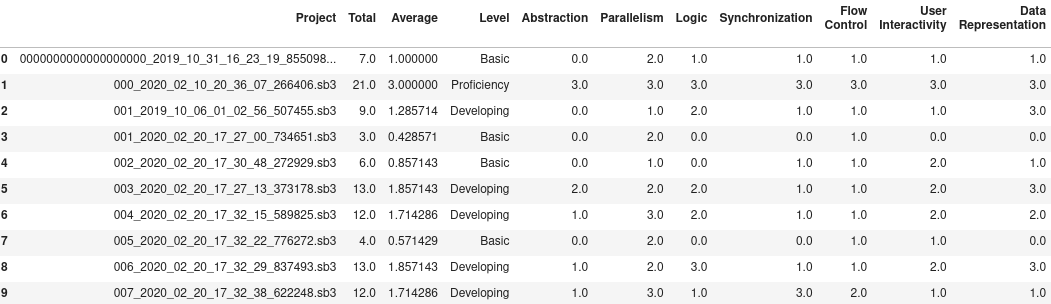
\includegraphics[width=1.0\textwidth]{img/df_origen_Scratch.png}
  	\caption{Dataframe de los proyectos de Scratch obtenido al cargar \emph{results.csv}}\label{fig:df_Scratch}
\end{figure}

Se comprueba que no existen proyectos de Scratch duplicados y se eliminan áquellos cuyas variables no tienen valores asignados. Como resultado se obtiene un dataset con 269842 proyectos. Se ajustan los tipos de las variables a discretas para las puntuaciones de cada dimensión y para la total, y de tipo categórico ordinal para los tres niveles que pueden alcanzar los proyectos de Scratch en función de su puntuación total: \emph{ básico o ``basic''} de 0 a 7 puntos, \emph{desarrollador o ``developing''} de 8 a 14 puntos y \emph{profesional o ``proficiency''} de 15 a 21 puntos. 
% Básico, en desarrollo y completo

\subsection{Análisis de los proyectos de Scratch por nivel o categoría asignada y puntuación total. Distribución de frecuencias}
\label{subsec:frec_nivel}

% Etapa de desarrollo del PC
Tras el preprocesamiento y limpieza de datos, se continúa con el análisis exploratorio de datos, en el que se responde a ¿cómo es la distribución de los proyectos de Scratch por nivel? 

% Proporción y comparaciones entre partes de un todo. Histograma para intervalos continuos, donde hay gaps o valores inusuales -> outliers
En los diagramas de barras y de sectores de la figura~\ref{fig:level_Scratch} se clasifican los proyectos de Scratch según la etapa de desarrollo en que se encuentren. La categoría ``\emph{basic}'' es la más frecuente pues agrupa 131007 proyectos que constituyen un 48,55\% del conjunto total. El siguiente nivel más frecuente es el intermedio o ``\emph{developing}'' con un 38,59\% del dataset completo, que se corresponde con 104142 proyectos. Únicamente 34689 proyectos de Scratch, un 12,86\% del total, alcanzan el nivel avanzado o ``\emph{proficiency}''. Aproximadamente la mitad de los proyectos de Scratch analizados son muy sencillos y no consiguen puntuar por encima de los 7 puntos totales. En contraste solo un 12,86\% demuestran un dominio del pensamiento computacional superior a los 14 puntos.

\begin{figure}[H]
	\centering
	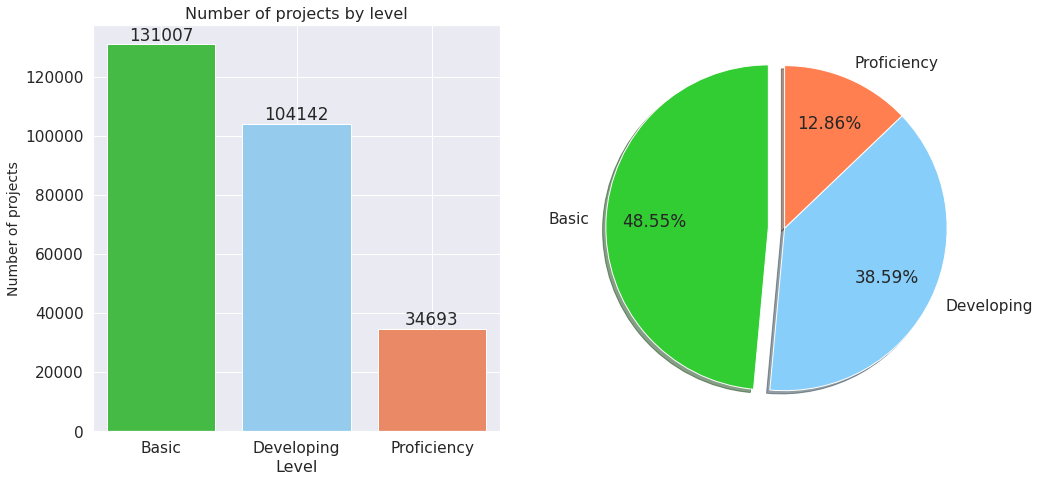
\includegraphics[width=1.0\textwidth]{img/freq_level_Scratch.png}
  	\caption{Distribución de proyectos de Scratch por nivel asignado}\label{fig:level_Scratch}
\end{figure}

¿Cómo se distribuyen los proyectos de Scratch entre las distintas puntuaciones asignadas a cada nivel?

Para la categoría \emph{basic} representada en la figura~\ref{fig:basic} se aprecia una tendencia ascendente en la puntuación conseguida, con un máximo en los 7 puntos. Si bien es importante remarcar que 16189 proyectos no consiguen puntuar por estar incompletos.

Sin embargo en la categoría intermedia o \emph{developing}, se sigue una tendencia descendente, como se observa en la figura~\ref{fig:developing}.

En la categoría de nivel avanzado o \emph{proficiency} se continúa con una tendencia descendente hasta los 18 puntos. Se eleva a 5570 la cantidad de proyectos con 19 puntos, para disminuir notablemente en los 21 puntos totales (véase figura~\ref{fig:proficiency}). Únicamente 180 proyectos obtienen la calificación máxima en cada una de las siete dimensiones del pensamiento computacional. 

\begin{figure}[H]
    \centering
    \begin{subfigure}[h]{.75\textwidth} 
        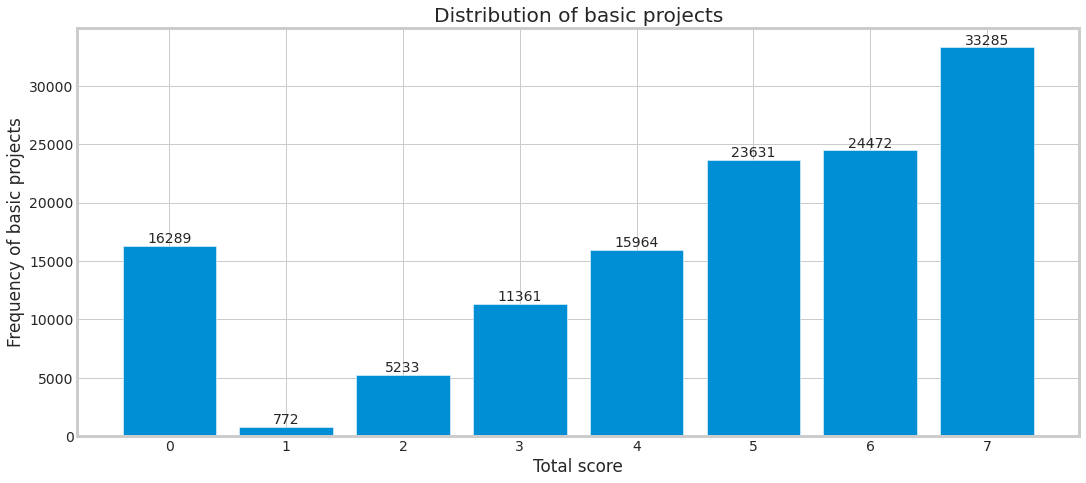
\includegraphics[width=\textwidth]{img/basic_Scratch}
        \caption{Nivel básico}
        \label{fig:basic}
    \end{subfigure}       
    \begin{subfigure}[h]{.75\textwidth} 
        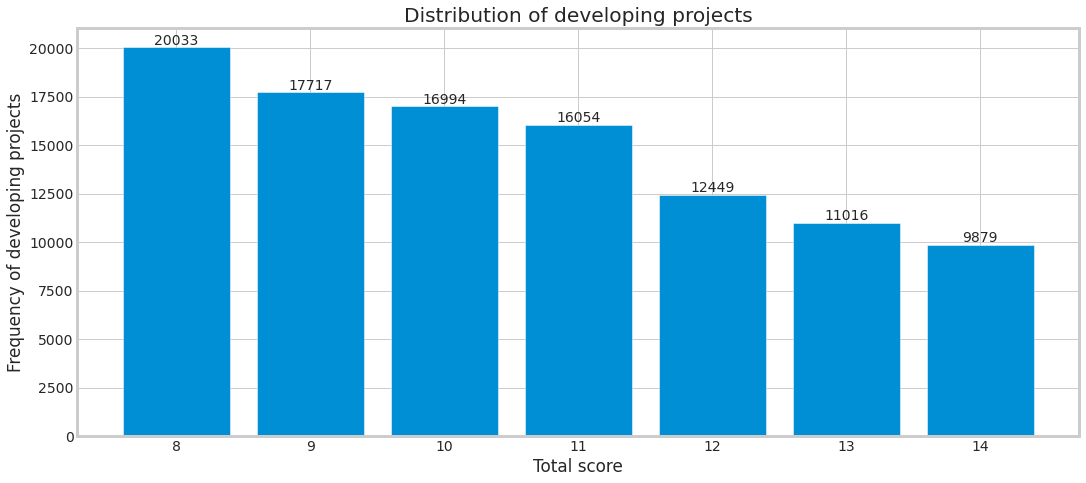
\includegraphics[width=\textwidth]{img/developing_Scratch}
        \caption{Nivel intermedio}
        \label{fig:developing}
    \end{subfigure}
    \begin{subfigure}[h]{.75\textwidth} 
        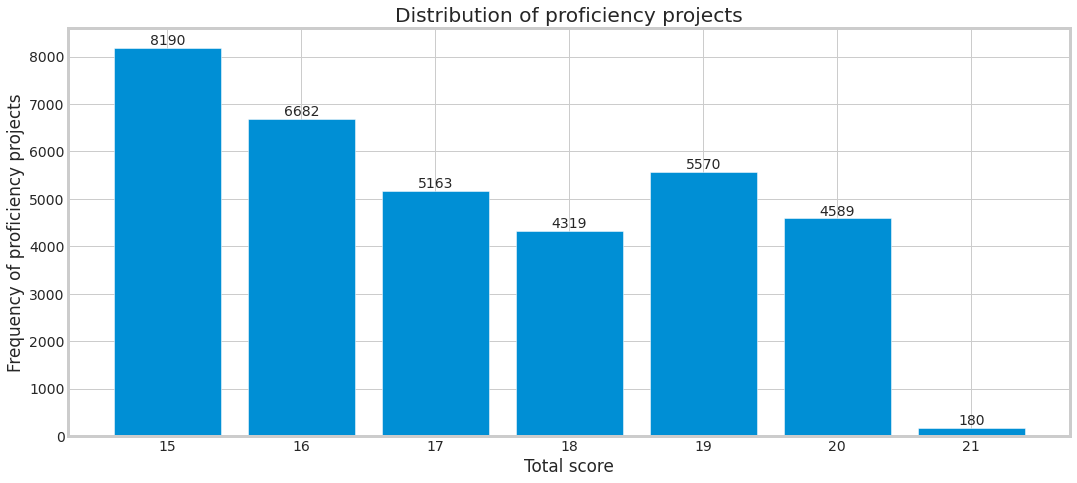
\includegraphics[width=\textwidth]{img/proficiency_Scratch}
        \caption{Nivel avanzado}
        \label{fig:proficiency}
    \end{subfigure}
    \caption{Distribución de proyectos de Scratch por puntuaciones asignadas a cada nivel}
\end{figure}

En la tabla~\ref{table:mean_Scratch} se indican las medidas de tendencia central y de dispersión para cada nivel. En el nivel \emph{basic}, al ser la media menor que la mediana, la distribución tiene una asimetría negativa o hacia la izquierda. En los niveles \emph{developing} y \emph{proficiency} la asimetría es positiva o hacia la derecha, puesto que la media supera a la mediana, aunque en los gráficos de distribución no es tan evidente. La dispersión de los valores de la puntuación con respecto a la media disminuye según aumenta el nivel, aunque se mantienen valores elevados de desviación típica para todos ellos, implicando que la mediana será más representativa que la media.

\begin{table}[htbp]
 \begin{center}
  \begin{tabular}{|c|c|c|c|c|}
    \hline
     \textbf{Nivel} & \textbf{Media} & \textbf{Mediana} & \textbf{Varianza} & \textbf{Desviación típica} \\ \hline
    \textbf{Basic} & 4.634554 & 5 & 5.100514 & 2.258432 \\ \hline
    \textbf{Developing} & 10.535164 & 10 & 3.755300 &  1.937860 \\ \hline
    \textbf{Proficiency} & 17.198426 & 17 & 3.137785 &  1.771379 \\ \hline
  \end{tabular}
  \caption{Medidas de tendencia central y dispersión para cada nivel.}
  \label{table:mean_Scratch}
 \end{center}
\end{table}

¿Cómo se distribuyen los proyectos de Scratch según la puntuación total?

Cómo se percibe en la figura~\ref{fig:total_Scratch}, se produce una elevada concentración de proyectos entre los 4 y los 11 puntos, con un máximo en los 7 puntos. La cantidad de proyectos que consiguen cada puntuación crece rápidamente hasta esta puntuación más frecuente o moda. A partir de la misma disminuye de manera más suave, obteniendo una cola que se extiende hacia la derecha según la valoración total del proyecto toma los valores más altos.

\begin{figure}[H]
	\centering
	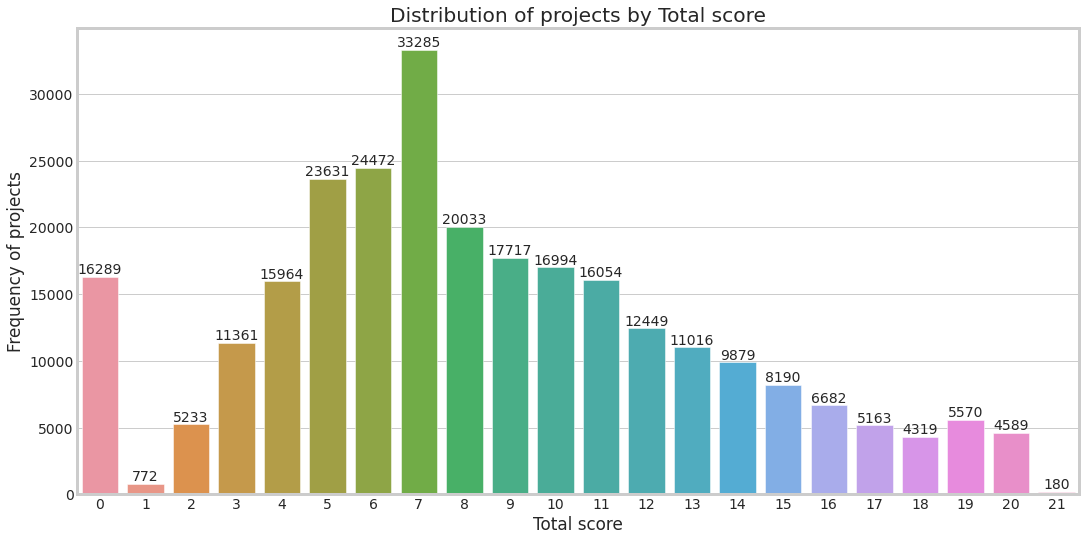
\includegraphics[width=.9
	\textwidth]{img/frequency_total_score_Scratch.png}
  	\caption{Distribución de proyectos de Scratch por puntuación total}\label{fig:total_Scratch}
\end{figure}

% Es normal que haya gran cantidad de proyectos de nivel basic puesto que los alumnos se inician en la programación y en el desarrollo de su pensamiento computacional con proyectos sencillos, para luego ir incrementando su complejidad, viéndose motivados por la realimentación que proporciona Dr. Scratch para mejorar en cada área y evitar malas prácticas. 
Parece razonable que aproximadamente la mitad de los proyectos se encuentren en un nivel básico con puntuaciones totales bajas, puesto que el público objetivo son alumnos que se inician en la programación y en el desarrollo de su pensamiento computacional con proyectos sencillos codificados en Scratch. La finalidad es que los alumnos incrementen la  complejidad de sus proyectos, al verse motivados por la realimentación que proporciona Dr. Scratch para mejorar en cada dimensión del pensamiento computacional y evitar malos hábitos al programar. La cantidad de proyectos que superen el umbral de los 7 puntos debería incrementarse para ascender a las categorías superiores. No obstante resulta complicado implementar proyectos que contengan todos los conceptos y prácticas computacionales de mayor valoración en cada dimensión.

\subsection{Frecuencia de los proyectos de Scratch por áreas del pensamiento computacional}
\label{subsec:frec_pc_Scratch}

¿Cuál es la distribución de la puntuación en cada dimensión?

% **Referenciar a la tabla en algún sitio o estado del arte dr. Scratch o diseño...
Se filtran y agrupan los proyectos según las métricas establecidas en Dr. Scratch para cada destreza del pensamiento computacional.

\begin{figure}[H]
    \centering      
    \begin{subfigure}[h]{1\textwidth} 
        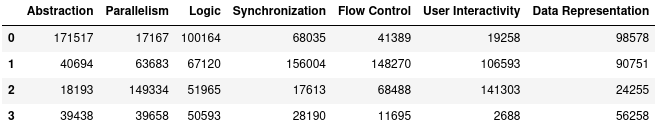
\includegraphics[width=\textwidth]{img/df_PC_Scratch.png}
        \caption{Dataframe con la cantidad de proyectos por puntuación y dimensión del PC}
        \label{fig:df_PC_Scratch}
    \end{subfigure}
    \begin{subfigure}[h]{1\textwidth} 
        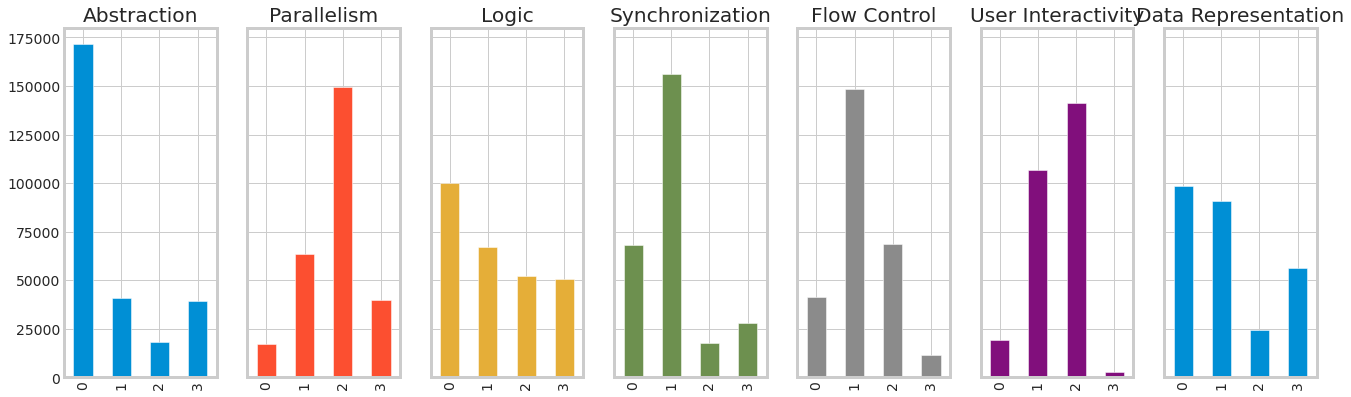
\includegraphics[width=\textwidth]{img/distribution_PC.png}
        \caption{Diagrama de barras con la cantidad de proyectos por puntuación y dimensión del PC}
        \label{fig:barras_PC_Scratch}
    \end{subfigure} 
\caption{Distribución de proyectos de Scratch por puntuación para cada dimensión del PC}
\end{figure}

% Lo que estaba en el cuaderno. Cambiado para que sea comparable con Snap! para cada CT
% Los peores resultados se obtienen en abstracción, donde 171517 proyectos tienen 0 puntos. Tanto en lógica como en representación de la información la frecuencia absoluta de la puntuación 0 es cercana a los 100000 proyectos, por lo que tampoco se consiguen buenos resultados en estas dimensiones, aunque en ellas las frecuencias están más repartidas entre las distintas puntuaciones. Tanto en sincronismo como en control de flujo del programa en torno a 150000 proyectos consiguen un punto. En paralelismo y en interactividad con el usuario la puntuación más frecuente es 2 puntos, siendo la puntuación de 1, la siguiente más frecuente.

\begin{itemize}
    
    \item \textbf{Abstracción}: Es la capacidad menos desarrollada. Se utiliza más de un script y más de un personaje u objeto en 40694 proyectos, estando evaluados con 1 punto. Los 3 puntos asignados por el uso de clones tienen una frecuencia absoluta similar, con 39438 proyectos. Únicamente 18193 proyectos tienen bloques o funciones definidas por el programador. Un total de 171517 proyectos carecen de estos elementos vinculados con la descomposición del problema en partes más sencillas que puedan ser reutilizadas tras extraer lo relevante de cada parte, descubrir patrones y generalizar.
    
    \item \textbf{Paralelismo}: La puntuación de 2 puntos destaca sobre las demás, con 149334 proyectos que cuentan con flujos de código que se ejecutan simultáneamente al pulsar sobre una tecla o sobre un objeto.
    
    \item \textbf{Pensamiento lógico}: En 100164 proyectos del dataset no se emplean estructuras condicionales que seleccionen las instrucciones a realizar en función de que se cumpla una condición. Un conjunto de 67120 proyectos cuentan con al menos un if, 51955 con un if-else y 50593 emplean operadores lógicos, disminuyendo la frecuencia según aumenta la complejidad.
    
    \item \textbf{Sincronización}: En 156004 proyectos se emplean bloques de espera para establecer el orden en que los programas de un proyecto se ejecutan, haciendo que interactúen entre sí, consiguiendo por ello 1 punto. Elementos como el intercambio de mensajes o establecer eventos de parada solo se utilizan en 17613 proyectos evaluados con 2 puntos. Aumenta la frecuencia de los que son valorados con 3 puntos por emplear eventos como el cambio de escenario o el resultado de la ejecución de otro programa para que se continúe con la ejecución de las sentencias sujetas a que se produzcan estos eventos.
    
    \item \textbf{Control de flujo}: En más de la mitad de los proyectos, en concreto en 148270, se demuestran nociones algorítmicas al secuenciar las instrucciones de manera concreta y precisa. Por ello obtienen un punto. La distribución se reduce linealmente, de modo que 68488 proyectos emplean bucles infinitos o que iteran un nº concreto de veces. Las estructuras iterativas sujetas a condiciones están presentes en 11695 proyectos, que reciben 3 puntos.
   
    % Videojuegos en cuenta los eventos que introduce el usuario en el programa
    \item \textbf{Interactividad con el usuario}: Se evalúa la gestión de las acciones que el usuario realiza sobre el programa cuando mueve el ratón, pulsa sobre los objetos, presiona teclas del teclado o responde a preguntas con 2 puntos, alcanzados en 141303 proyectos. La siguiente valoración más frecuente es 1 punto, con 106593 proyectos que solo cuentan con la bandera verde como elemento interactivo que desencadena la ejecución de los programas.
    
    \item \textbf{Representación de la información}: Se modifican los atributos de los objetos o personajes en 90751 proyectos, que obtienen un punto. Llama la atención la escasez de proyectos que consiguen 2 puntos por inicializar y modificar variables para almacenar los datos que requieren los programas, frente a los 56258 que utilizan listas y sus métodos, siendo calificados con la máxima puntuación. % como contenedores de múltiples datos de diferente tipo
    
\end{itemize}

\subsection{Análisis estadístico general de las dimensiones del pensamiento \\computacional con Scratch}
\label{subsec:estad_pc_Scratch}

% Estos resultados guardan consonancia con lo que se refleja en la figura~\ref{fig:barras_PC_Scratch}.
Se complementa el análisis univariante calculando los estadísticos descriptivos más básicos para cada capacidad que se muestran en la figura~\ref{fig:describe_Scratch}. A partir del valor medio y de la medida de posición del segundo cuartil, que coincide con la mediana, se infiere que las habilidades más desarrolladas son paralelismo e interactividad con el usuario, mientras que abstracción es la que resulta más compleja. Su dispersión en torno a la media es una de las más altas, junto a la que se produce en representación de los datos y pensamiento lógico. El 75\% de los proyectos son valorados con 0 o 1 puntos en abstracción y sincronización, mientras que para el resto de dimensiones algunos de ellos alcanzan los 2 puntos. 

\begin{figure}[H]
	\centering
	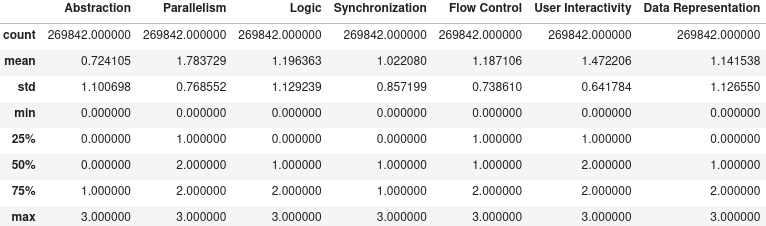
\includegraphics[width=1\textwidth]{img/describe_Scratch.png}
  	\caption{Media, desviación estándar y cuartiles de cada CT}\label{fig:describe_Scratch}
\end{figure}

A continuación se representa en la figura~\ref{fig:cajas_Scratch} la concentración de las puntuaciones de cada habilidad del PC en base a la mediana y a los cuartiles y se comprueba si existen valores atípicos.

\begin{figure}[H]
	\centering
	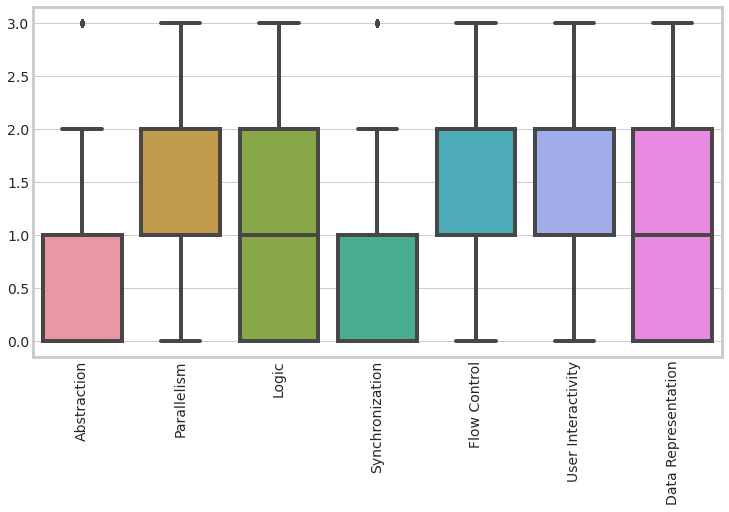
\includegraphics[width=0.7\textwidth]{img/diag_cajas_Scratch2.png}
  	\caption{Diagrama de cajas de cada dimensión del CT}\label{fig:cajas_Scratch}
\end{figure}

\begin{itemize}
    \item \textbf{Abstracción y sincronización}: Al ordenar los proyectos de menor a mayor puntuación más de la mitad no puntúan en abstracción. Por lo tanto el primer cuartil $(Q_1)$ y la mediana están situados en 0. En el tercer cuartil $(Q_3)$ algunos proyectos consiguen 1 punto. En sincronización la mediana coincide con el tercer cuartil en 1 punto. En ambos el 75\% de los proyectos están entre 0 y 1 puntos, el límite superior se localiza en los 2 puntos y los proyectos con 3 puntos serían \emph{outliers} o valores atípicos, pero válidos en este estudio, ya que hay más proyectos con 3 puntos que con 2 puntos, como se veía en la  figura~\ref{fig:df_PC_Scratch}.
    \item \textbf{Paralelismo, interactividad con el usuario y control de flujo}: Sus diagramas de cajas son similares y las distribuciones son más simétricas. Los proyectos alcanzan 1 punto en el primer cuartil y 2 puntos en el tercer cuartil. La mediana de paralelismo e interactividad con el usuario coincide con el tercer cuartil y se corresponde con los 2 puntos. En cambio, para control de flujo la mediana coincide con el primer cuartil en 1 punto. El límite superior para las tres está en 3 puntos. Todo ello indica que las puntuaciones están más concentradas en 1 y 2 puntos, con mayor cantidad de proyectos en el cuartil que coincide con la mediana.
    \item\textbf{Pensamiento lógico y representación de los datos}: También siguen una dispersión similar, con un rango intercuartil de 0 a 2 puntos y la mediana en 1 punto. Sus valores están más dispersos que en las otras dimensiones. El límite superior está en 3 puntos. 
\end{itemize}

%Tendría sentido meter cv de Pearson y media y std para cada dimensión y nivel?
Siguiendo con el análisis exploratorio de datos o EDA se calculan los coeficientes de correlación de Pearson existentes entre la puntuación total y las distintas habilidades, para determinar si existe una dependencia lineal perfecta o próxima a 1.% y el aporte de cada una. función lineal que una la variable x con la variable Y


\begin{table}[htbp]
 \begin{center}
 \resizebox{15cm}{!} {
    \begin{tabular}{|c|c|c|c|c|c|c|c|}
	\hline
	\textbf{Correlación} & \textbf{Abstracción} & \textbf{Paralelismo} & \textbf{Lógica} & \textbf{Sincronización} & \textbf{Control de flujo} & \textbf{\begin{tabular}[c]{@{}c@{}}Interactividad\\ con el usuario\end{tabular}} & \textbf{\begin{tabular}[c]{@{}c@{}}Representación\\ de los datos\end{tabular}} \\
	\hline
	\textbf{Total} & 0.772359 & 0.720550 &  0.787795 & 0.753190 & 0.772396 & 0.609517 &  0.786001 \\
	\hline
    \end{tabular} }
    \caption{Correlación de la puntuación total con cada dimensión del PC}
    \label{table:corr_total_Scratch}
 \end{center}
\end{table}

De la tabla~\ref{table:corr_total_Scratch} se deduce que las correlaciones son directas y fuertes entre la puntuación total y cada dimensión del pensamiento computacional, al ser superiores a 0.7,
%$\rho>0.7$**, 
salvo en interactividad con el usuario, que sería la habilidad que menos aporta a la puntuación total y la que más información contiene. Cuando aumenta la puntuación de interactividad se incrementa la puntuación total en menor medida que si crecen las valoraciones de las otras dimensiones.
    
El siguiente paso es indagar si existen relaciones entre las dimensiones del pensamiento computacional o si por el contrario son todas independientes linealmente entre sí. Para ello se realiza un análisis multivariante, calculando la correlación de Pearson para cada par de características o dimensiones. % Si dos de ellas son dependientes se podrían agrupar  % Herramienta fundamental del EDA

\begin{figure}[H]
	\centering
  	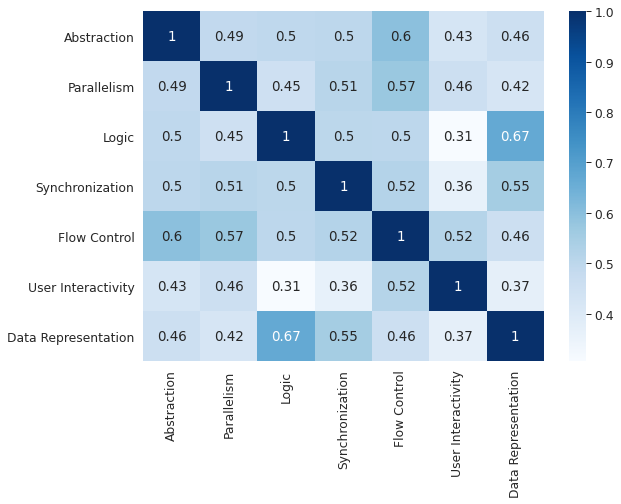
\includegraphics[width=.7\textwidth]{img/corr_Scratch.png}
  	\caption{Matriz de correlación de Pearson de las dimensiones del PC.}\label{fig:corr_Scratch}
\end{figure}

Se producen correlaciones positivas débiles y moderadas entre cada par de dimensiones. Las más bajas ocurren entre interactividad con el usuario con cada una de las siguientes: lógica, sincronización y representación de la información. Existe escasa dependencia entre implementar código que se encargue de las acciones que realice el usuario sobre el programa con determinar las sentencias que se ejecutan en función de condiciones, con la organización de la ejecución de los distintos programas de manera que interactúen entre sí y con la declaración y la modificación de los datos sobre los que se opera en los programas.

%Que la interactividad con el usuario guarde escasa relación con el resto de dimensiones del pensamiento computacional es perfectamente comprensible ya que los 3 puntos se consiguen únicamente porque el usuario emplee el micrófono o la cámara y esto no requiere el uso de otra destreza del pensamiento computacional.

Los mayores coeficientes de correlación, que se corresponden con una correlación positiva moderada, se obtienen entre:

\begin{itemize}
    \item \textbf{Lógica y representación de los datos}: Cuando se codifican estructuras algorítmicas selectivas, planteando las condiciones que determinan por dónde continúa el flujo del programa, también aumenta la habilidad para definir y manipular los datos de variables, listas y atributos que necesitan los personajes y programas para su ejecución.
    \item \textbf{Abstracción y control de flujo}: La destreza mostrada al descomponer en partes el problema a resolver con funciones y procedimientos encargados de tareas concretas e instanciando objetos o clones cuando se requiera que hagan las mismas instrucciones, guarda relación con las nociones algorítmicas demostradas en cada una de esas partes ya sea secuenciando instrucciones o empleando bucles. %%
    \item \textbf{Paralelismo y control de flujo}: La capacidad de dividir el problema en programas que son ejecutados a la vez por uno o varios personajes depende linealmente de que los algoritmos que sustentan dichos programas estén definidos de manera precisa y ordenada y utilicen bucles cuando sea recomendable.
    \item \textbf{Sincronización y representación de los datos}: Establecer el orden en que se ejecutan los distintos programas para que interactúen entre sí se relaciona con declarar y modificar las variables, listas y atributos que contienen los datos requeridos en todos ellos.
\end{itemize}


\subsection{Frecuencias y correlaciones de las dimensiones del PC en función de la puntuación total para proyectos de Scratch}
\label{subsec:corr_21_Scratch}

Se profundiza en el análisis multivariante comprobando las dependencias lineales entre cada par de dimensiones del pensamiento computacional según aumenta la puntuación total. Para ello se observa la evolución de la matriz de correlación de Pearson y de las distribuciones de puntuación en cada dimensión. El objetivo es tratar de esclarecer cuáles son las dimensiones que se desarrollan antes, qué puntuaciones se les van asignando y qué relaciones se establecen entre ellas según aumenta la complejidad de los proyectos, determinada por la puntuación total.

\begin{figure}[H]
    \centering
    \begin{subfigure}[h]{.49\textwidth} 
        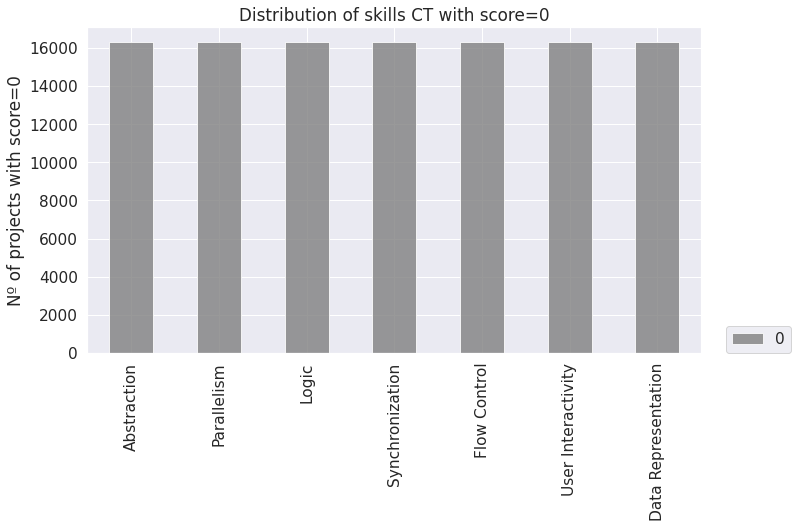
\includegraphics[width=\textwidth]{img/distribucion_0_Scratch}
        \caption{Puntuación total = 0}
        \label{fig:total0}
    \end{subfigure}       
    \begin{subfigure}[h]{.49\textwidth} 
        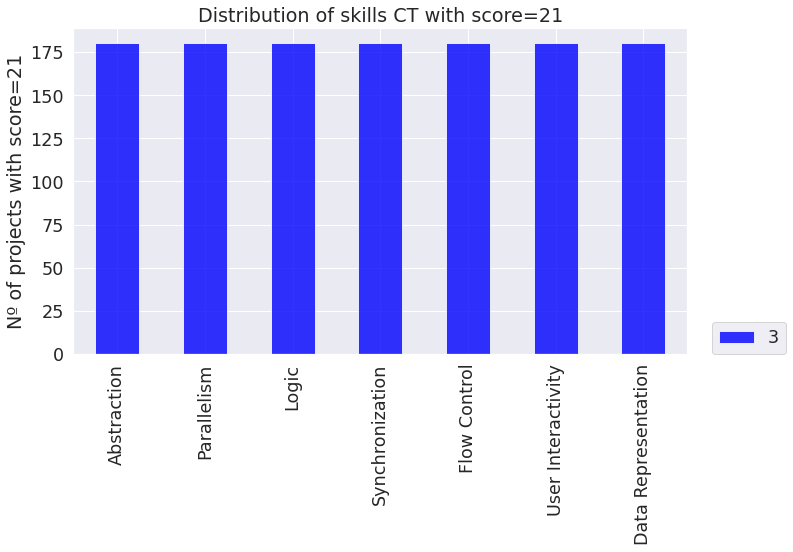
\includegraphics[width=\textwidth]{img/distribucion_21_Scratch}
        \caption{Puntuación total = 21}
        \label{fig:total21}
    \end{subfigure}
     \caption{Distribución de proyectos de Scratch para cada habilidad del PC para las puntuaciones totales mínima y máxima}
\end{figure}

 Como paso previo se examinan las distribuciones de las puntuaciones totales de las figuras~\ref{fig:total0} y ~\ref{fig:total21}, que están sometidas a particularidades. En los casos extremos, cuando la puntuación total es de 0 y 21, todas las dimensiones tienen asignadas las mismas puntuaciones en cada proyecto, 0 y 3 respectivamente. No hay dispersión con respecto a la media, tanto al tomar cada variable o dimensión por separado como al analizar la variación conjunta de cada par de variables. Por lo tanto la covarianza y la raíz de la varianza o desviación típica son nulas y su razón, que conforma el coeficiente de correlación, indeterminada (véase la ecuación~\eqref{eq:correlacion}). % variación conjunta con respecto a las medias

\begin{equation}
   \rho_{xy} = \dfrac{Cov(X,Y)}{\sigma_{x}\sigma_{y}} = \dfrac{\sum_{i=1}^{n} (x_i - \overline{x})(y_i - \overline{y})}{\sqrt{\sum_{i=1}^{n} (x_i - \overline{x})^{2}}\sqrt{\sum_{i=1}^{n} (y_i - \overline{y})^{2}}},  siendo: -1<\rho_{xy}<1
   \label{eq:correlacion}
\end{equation}   

Se prosigue con el desglose de las puntuaciones conseguidas en cada habilidad para cada puntuación total, según progresa de 1 a 20 y se analizan las dependencias que surgen entre ellas.

Si la puntuación total es 1 aumenta paralelismo e interactividad con el usuario, y en menor medida control de flujo y sincronización, según vemos en el diagrama de barras~\ref{fig:total1}. Las dos primeras son las capacidades que se desarrollan cuando los programadores comienzan a utilizar  Scratch. Al repartirse el punto entre varias dimensiones,
la matriz de correlación~\ref{fig:corr1} muestra una correlación perfecta positiva para cada par de dimensiones del pensamiento computacional.

\begin{figure}[H]
    \centering
    \begin{subfigure}[h]{.49\textwidth} 
        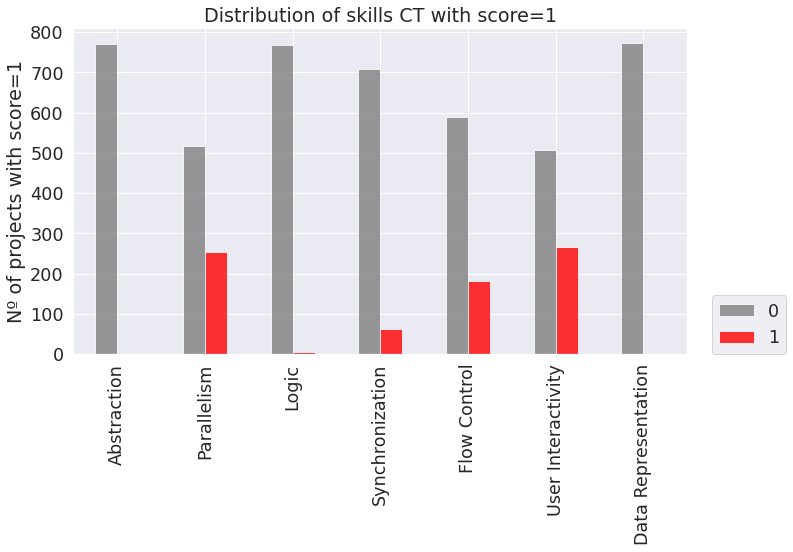
\includegraphics[width=\textwidth]{img/distribucion_1_Scratch}
        \caption{Diagrama de barras. Total=1}
        \label{fig:total1}
    \end{subfigure}       
    \begin{subfigure}[h]{.49\textwidth} 
        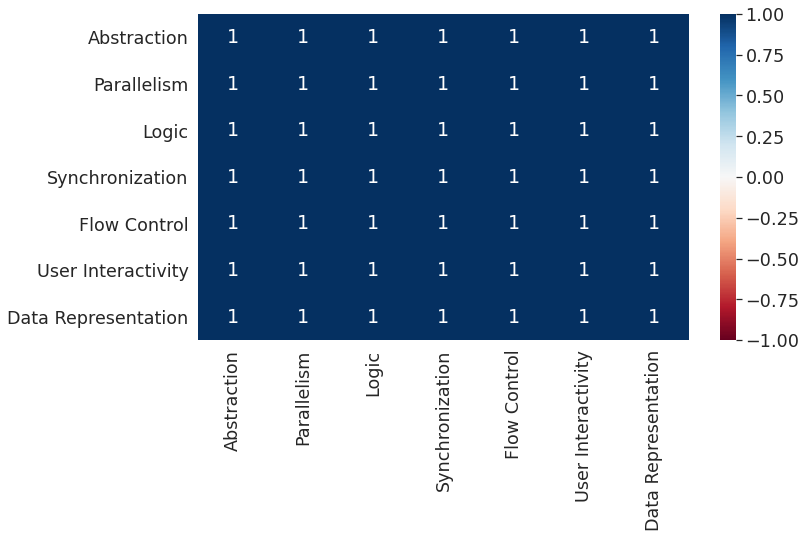
\includegraphics[width=\textwidth]{img/corr_1_Scratch}
        \caption{Matriz de correlación. Total=1}
        \label{fig:corr1}
    \end{subfigure}
     \caption{Distribución de puntuaciones asignadas y correlación entre dimensiones del PC cuando la puntuación total vale 1}
\end{figure}

\begin{figure}[H]
    \centering
    \begin{subfigure}[h]{.49\textwidth} 
        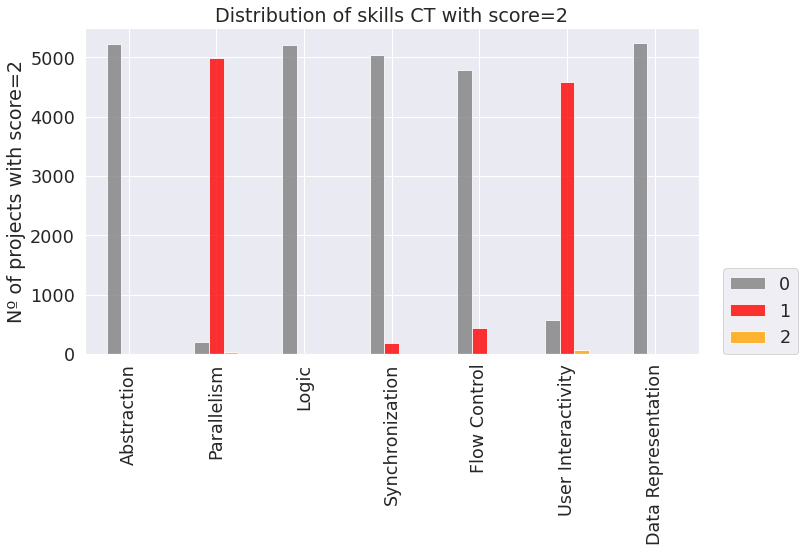
\includegraphics[width=\textwidth]{img/distribucion_2_Scratch}
        \caption{Diagrama de barras. Total=2}
        \label{fig:total2}
    \end{subfigure}       
    \begin{subfigure}[h]{.49\textwidth} 
        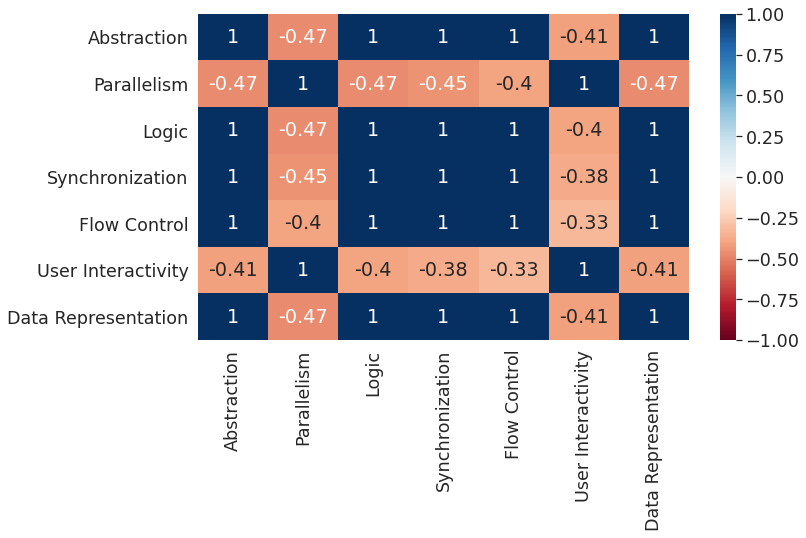
\includegraphics[width=\textwidth]{img/corr_2_Scratch}
        \caption{Matriz de correlación. Total=2}
        \label{fig:corr2}
    \end{subfigure}
     \caption{Distribución de puntuaciones asignadas y correlación entre dimensiones del PC cuando la puntuación total vale 2}
\end{figure}

Como se percibe en la figura~\ref{fig:total2} la mayor parte de los proyectos cuentan con 1 punto en paralelismo y en interactividad con el usuario, que agregados conforman el total de 2.

De la matriz de correlación de la figura~\ref{fig:corr2} se deduce que aquellos pares de variables en los que la correlación no es perfecta y positiva, tienen una correlación débil y negativa. Entre paralelismo e interactividad con el usuario se produce una dependencia lineal perfecta, ya que cuando el usuario pulsa la bandera verde se desencadena la ejecución de varios flujos de código simultáneamente. Estas dos dimensiones se relacionan en sentido inverso con las otras aptitudes. El resto de dimensiones mantienen entre sí una relación perfecta positiva porque no puntúan. 

\begin{figure}[H]
    \centering
    \begin{subfigure}[h]{.49\textwidth} 
        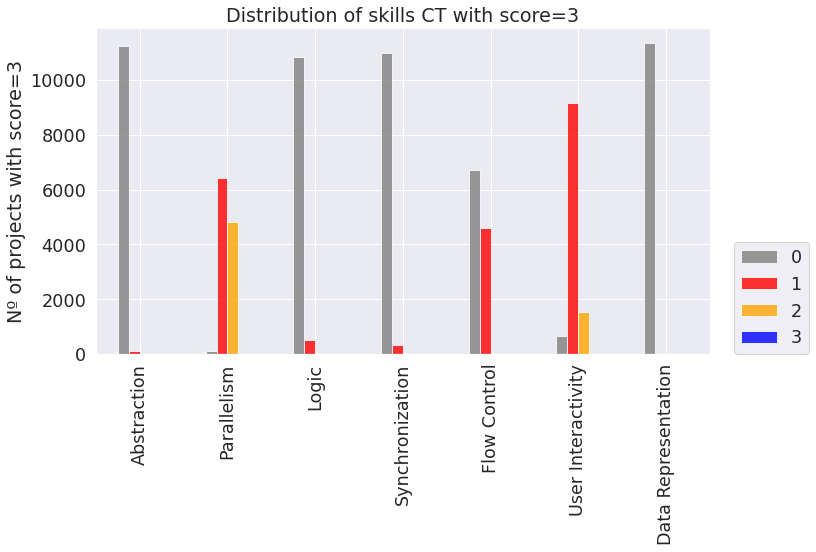
\includegraphics[width=\textwidth]{img/distribucion_3_Scratch}
        \caption{Diagrama de barras. Total=3}
        \label{fig:total3}
    \end{subfigure}       
    \begin{subfigure}[h]{.49\textwidth} 
        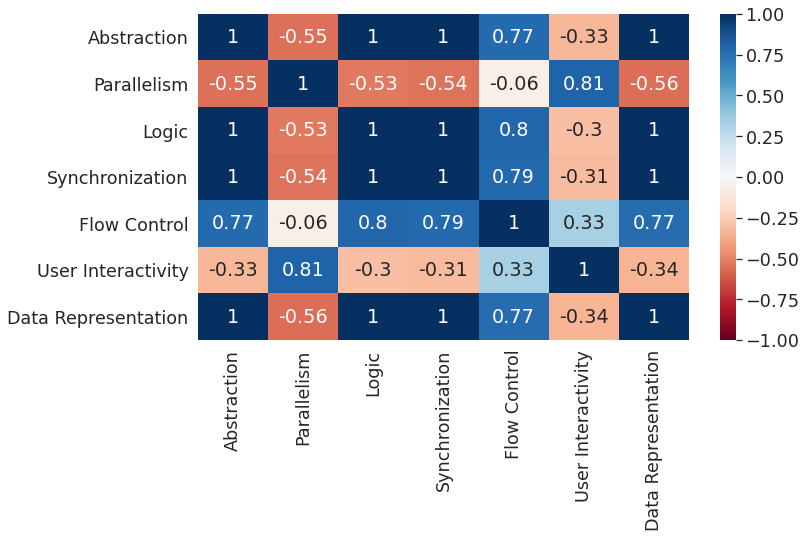
\includegraphics[width=\textwidth]{img/corr_3_Scratch}
        \caption{Matriz de correlación. Total=3}
        \label{fig:corr3}
    \end{subfigure}
     \caption{Distribución de puntuaciones asignadas y correlación entre dimensiones del PC cuando la puntuación total vale 3}
\end{figure}

En la figura~\ref{fig:total3} se observa que los proyectos completan los 3 puntos totales con 1 o 2 puntos en paralelismo, 1 punto en interactividad con el usuario o incluso 1 punto en control de flujo, puesto que la frecuencia de ocurrencia es superior a 4000.

Persisten las dependencias lineales positivas perfectas, con $\rho=1$, entre las capacidades con valoración nula, como se constata en la figura~\ref{fig:corr3}. Entre paralelismo e interactividad con el usuario hay una correlación positiva alta, igual que entre control de flujo y lógica y entre control de flujo y sincronización. No hay dependencia lineal entre control de flujo y paralelismo. Hay una correlación negativa moderada entre paralelismo con: representación de los datos, abstracción, lógica o sincronización. Es extraño que según aumenta una de las variables disminuya la otra, ya que el aumento en la capacidad para realizar tareas simultáneamente, no tiene por qué disminuir a la capacidad para establecer los atributos de los distintos objetos del proyecto o la habilidad para subdividir el problema en partes o ser capaz de establecer las condiciones que determinan la ejecución de unas acciones u otras. El hecho de que según aumenta paralelismo disminuya sincronización es bastante contradictorio, pues si se realizan tareas simultáneas debe existir alguna forma de que ajusten su ejecución en el tiempo.

En el diagrama de barras~\ref{fig:total4} se ve que en abstracción, lógica, sincronización y representación de los datos se siguen obteniendo 0 puntos en la mayoría de los proyectos. Sin embargo, se incrementan los que consiguen 1 punto en lógica, en sincronización y en control de flujo.

En la matriz de correlación~\ref{fig:corr4} queda patente que  existe dependencia lineal casi perfecta entre las dimensiones cuya puntuación más frecuente es 0 puntos. Cuando se codifican programas interactivos aumentan las nociones algorítmicas, como se deduce de la elevada relación lineal directa entre interactividad con el usuario y control de flujo. No existe dependencia lineal entre representación de los datos y control de flujo, ni entre este último y abstracción. Existe una correlación negativa moderada entre paralelismo y abstracción. El aumento de la valoración en una de las habilidades no debería hacer disminuir la otra. De hecho, la descomposición del programa en subprogramas encargados de tareas concretas podría facilitar la ejecución simultánea de varios subprogramas. También se da este tipo de correlación negativa entre paralelismo y representación de los datos.%%

\begin{figure}[H]
    \centering
    \begin{subfigure}[h]{.49\textwidth} 
        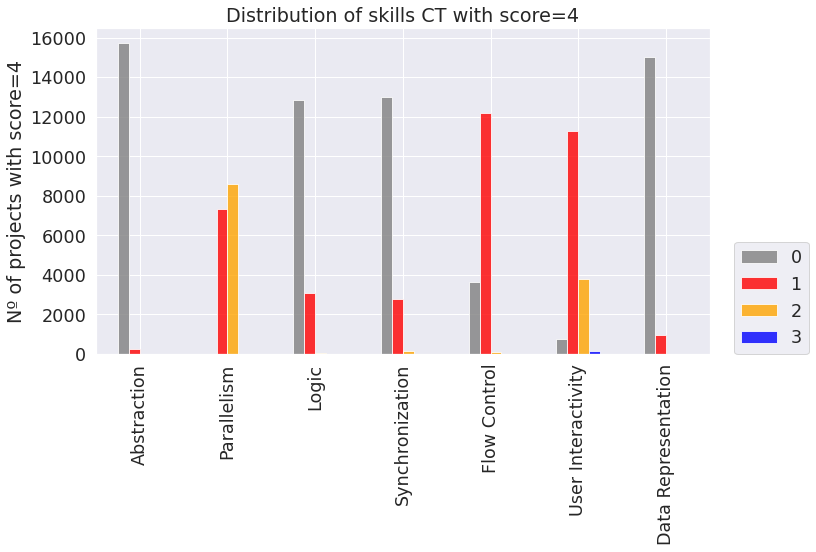
\includegraphics[width=\textwidth]{img/distribucion_4_Scratch}
        \caption{Diagrama de barras. Total=4}
        \label{fig:total4}
    \end{subfigure}       
    \begin{subfigure}[h]{.49\textwidth} 
        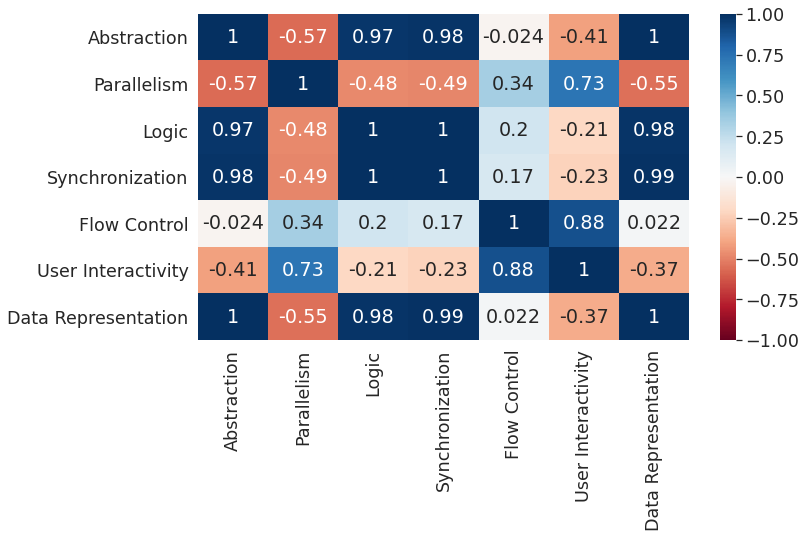
\includegraphics[width=\textwidth]{img/corr_4_Scratch}
        \caption{Matriz de correlación. Total=4}
        \label{fig:corr4}
    \end{subfigure}
     \caption{Distribución de puntuaciones asignadas y correlación entre dimensiones del PC cuando la puntuación total vale 4}
\end{figure}


Según el diagrama de barras~\ref{fig:total5} correspondiente a la puntuación total de 5, paralelismo e interactividad con el usuario son las capacidades mejor valoradas, puesto que la mitad de los proyectos consiguen 2 puntos. También aumenta la cantidad de proyectos que consiguen 1 punto en lógica y sincronización.

Al aumentar las puntuaciones, hay menos pares de dimensiones con coeficiente de correlación perfecto. Las máximas correlaciones en sentido positivo se producen entre paralelismo e interactividad con el usuario, y en menor medida entre representación de los datos y abstracción, entre sincronización y lógica y entre representación de los datos y lógica, como se observa en la figura~\ref{fig:corr5}. Resulta llamativo que no exista correlación entre sincronización y paralelismo, ya que si se ejecutan varios conjuntos de bloques a la vez tiene que existir algún evento que sincronice los procesos de manera que se comuniquen entre sí. Vuelve a aparecer una correlación moderada en sentido negativo entre paralelismo y abstracción con el mismo coeficiente que en la puntuación total de 4 puntos. También se obtiene una correlación de este tipo entre interactividad con el usuario y abstracción.%%

\begin{figure}[H]
    \centering
    \begin{subfigure}[h]{.49\textwidth} 
        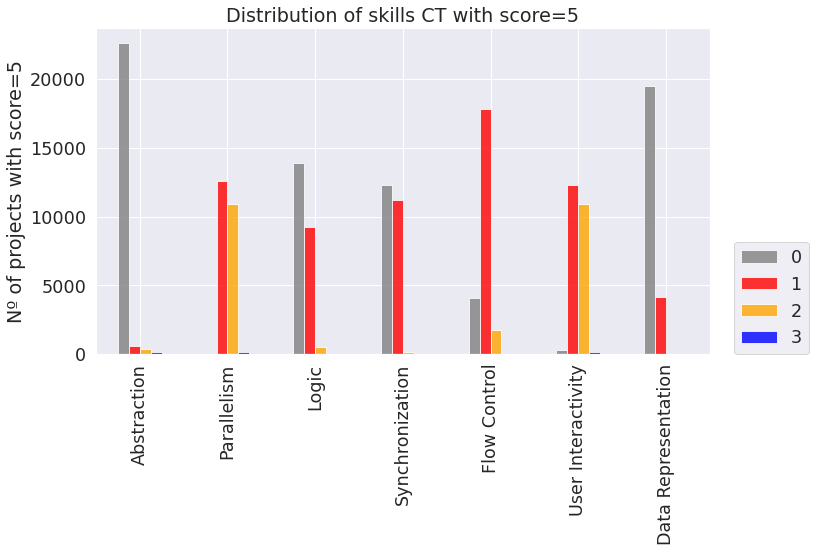
\includegraphics[width=\textwidth]{img/distribucion_5_Scratch}
        \caption{Diagrama de barras. Total=5}
        \label{fig:total5}
    \end{subfigure}       
    \begin{subfigure}[h]{.49\textwidth} 
        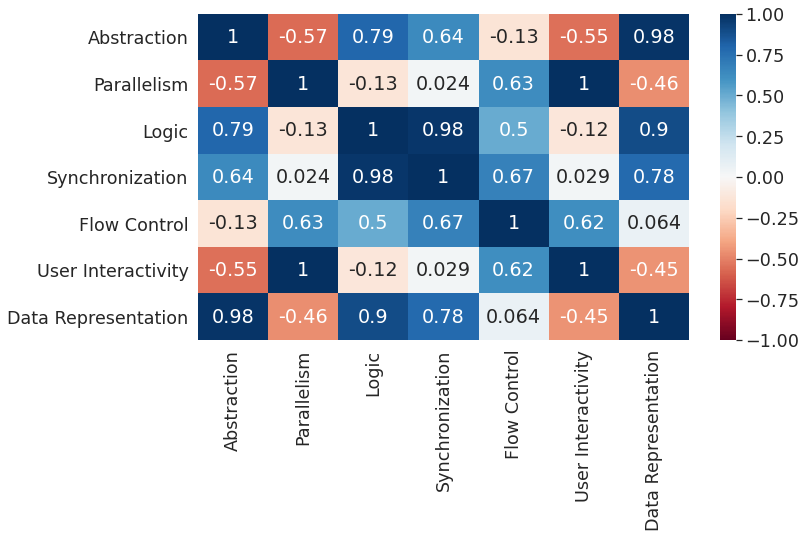
\includegraphics[width=\textwidth]{img/corr_5_Scratch}
        \caption{Matriz de correlación. Total=5}
        \label{fig:corr5}
    \end{subfigure}
     \caption{Distribución de puntuaciones asignadas y correlación entre dimensiones del PC cuando la puntuación total vale 5}
\end{figure}

Según se distingue en el diagrama de barras~\ref{fig:total6} correspondiente a la puntuación total de 6, se eleva la cantidad de proyectos con 1 punto en sincronización, control de flujo, interactividad con el usuario y representación de los datos.

Paralelismo y abstracción obtienen una correlación moderada en sentido negativo similar a la puntuación anterior. No hay correlación entre abstracción y sincronización, ni entre paralelismo y representación de los datos. Las mayores correlaciones se obtienen entre: control de flujo y sincronización, de modo que la secuenciación precisa, concreta y ordenada de instrucciones o bloques afecta a la organización temporal de los distintos flujos de código para que interactúen entre sí; entre lógica y representación de los datos, ya que tener una alta capacidad para buscar la solución al problema e implementar distintas acciones en función de condiciones, influye en almacenar en atributos y variables los datos tanto de condiciones como de resultados. Entre paralelismo e interactividad con el usuario existe una alta  dependencia ya que el usuario puede pulsar sobre una tecla u objeto provocando la ejecución simultánea de varias secuencias de bloques.%%

\begin{figure}[H]
    \centering
    \begin{subfigure}[h]{.49\textwidth} 
        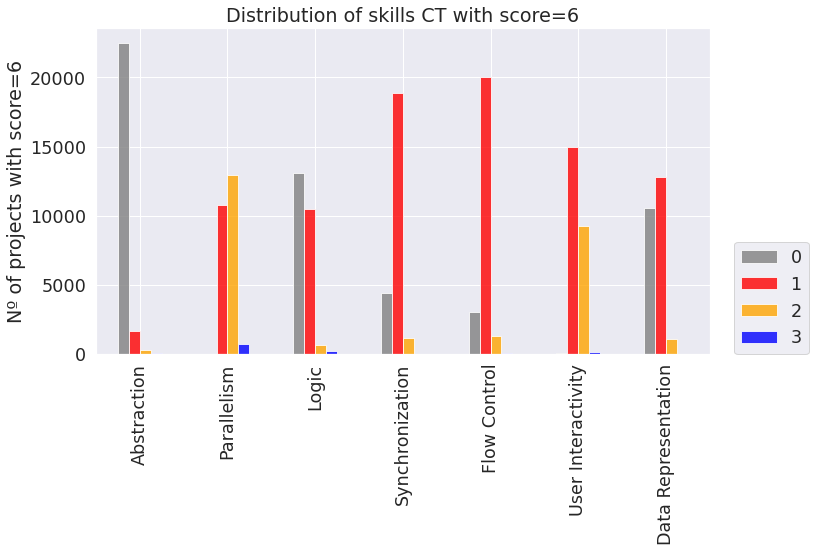
\includegraphics[width=\textwidth]{img/distribucion_6_Scratch}
        \caption{Diagrama de barras. Total=6}
        \label{fig:total6}
    \end{subfigure}       
    \begin{subfigure}[h]{.49\textwidth} 
        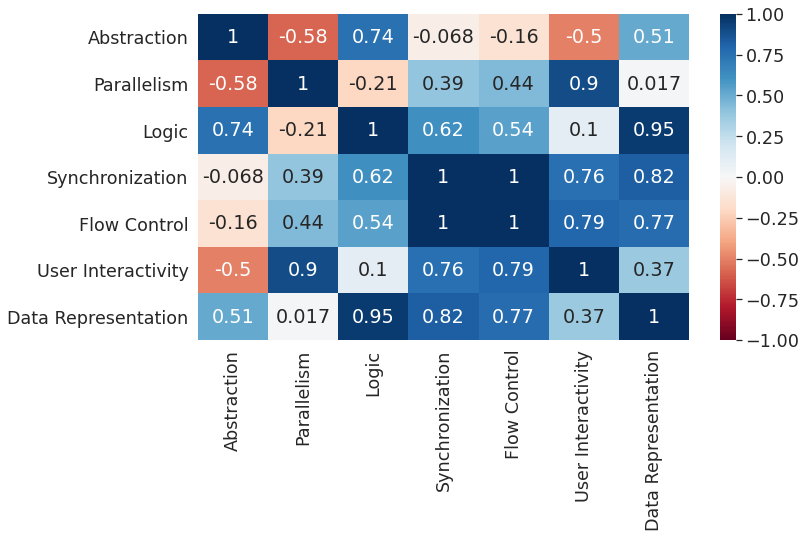
\includegraphics[width=\textwidth]{img/corr_6_Scratch}
        \caption{Matriz de correlación. Total=6}
        \label{fig:corr6}
    \end{subfigure}
     \caption{Distribución de puntuaciones asignadas y correlación entre dimensiones del PC cuando la puntuación total vale 6}
\end{figure}

Para la puntuación total de 7, lo más destacable en la representación de frecuencias de la figura~\ref{fig:total7} es que el nº de proyectos con una puntuación de 2 en paralelismo aumenta.

La correlación es perfecta positiva entre control de flujo y sincronización y entre lógica y representación de los datos, como se visualiza en la matriz~\ref{fig:corr7}. Se alcanzan valores elevados entre lógica y sincronización, representación de los datos y sincronización, control de flujo y lógica, interactividad con el usuario y control de flujo y entre interactividad con el usuario y sincronización. Que no exista correlación entre sincronización y paralelismo resulta contradictorio, ya que si se ejecutan flujos de código a la vez debería desarrollarse la capacidad de sincronizarlos, aunque no precisamente con el bloque de espera evaluado con 1 punto. Tampoco existe correlación entre abstracción y representación de los datos, puesto que aún no se ha desarrollado la capacidad de dividir el problema en partes más simples. % hasta esta puntuación total. % Esto implica que ser capaz de codificar scripts encargados de tareas concretas que resuelvan en conjunto un problema complejo, ejecutados por los  personajes del proyecto, no influye en cómo se modifiquen sus atributos.%% modularidad y abstracción de datos 0 puntos


\begin{figure}[H]
    \centering
    \begin{subfigure}[h]{.49\textwidth} 
        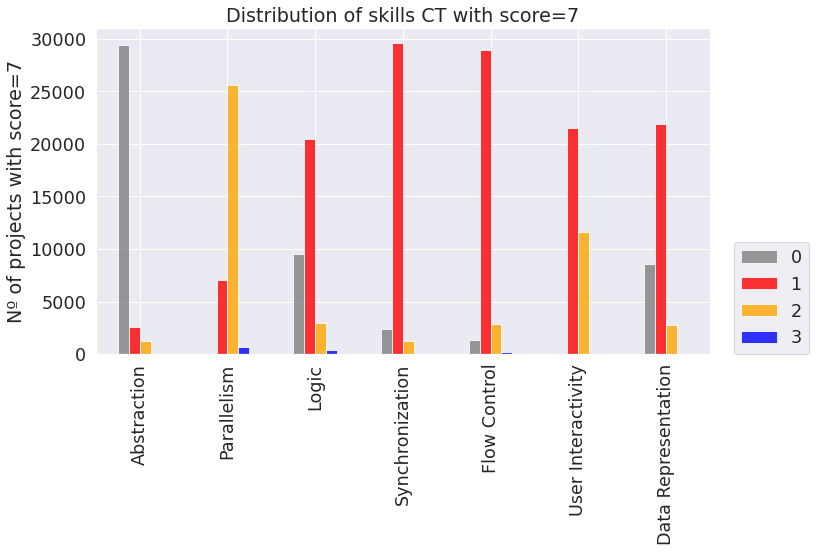
\includegraphics[width=\textwidth]{img/distribucion_7_Scratch}
        \caption{Diagrama de barras. Total=7}
        \label{fig:total7}
    \end{subfigure}       
    \begin{subfigure}[h]{.49\textwidth} 
        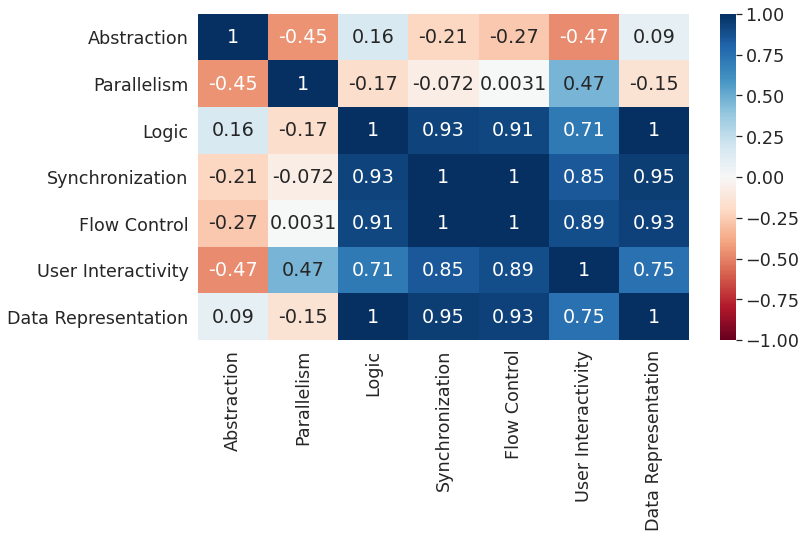
\includegraphics[width=\textwidth]{img/corr_7_Scratch}
        \caption{Matriz de correlación. Total=7}
        \label{fig:corr7}
    \end{subfigure}
     \caption{Distribución de puntuaciones asignadas y correlación entre dimensiones del PC cuando la puntuación total vale 7}
\end{figure}

\begin{figure}[H]
    \centering
    \begin{subfigure}[h]{.49\textwidth} 
        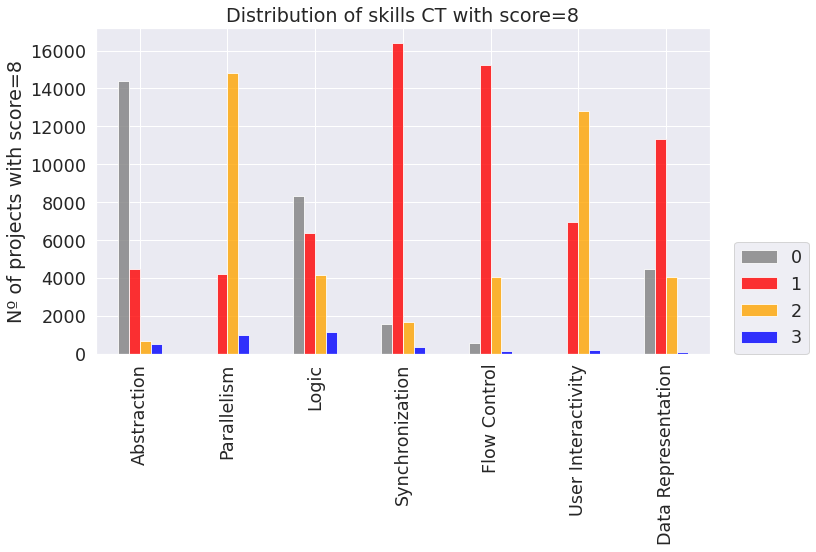
\includegraphics[width=\textwidth]{img/distribucion_8_Scratch}
        \caption{Diagrama de barras. Total=8}
        \label{fig:total8}
    \end{subfigure}       
    \begin{subfigure}[h]{.49\textwidth} 
        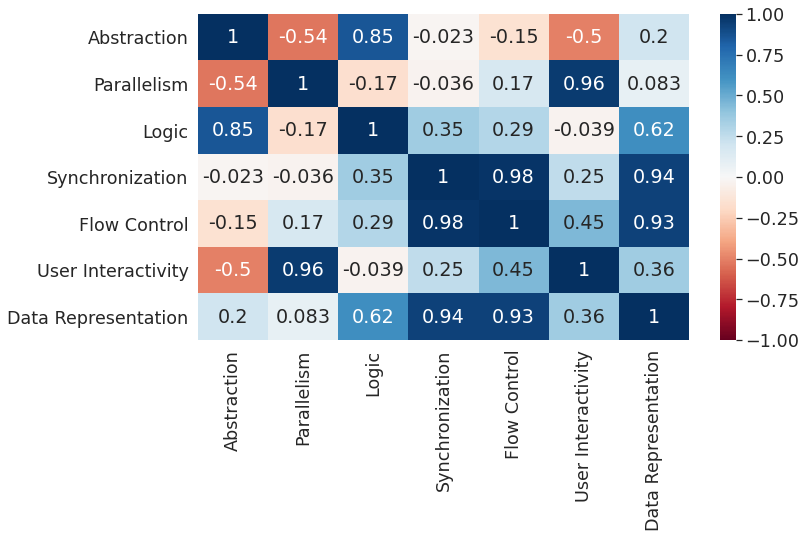
\includegraphics[width=\textwidth]{img/corr_8_Scratch}
        \caption{Matriz de correlación. Total=8}
        \label{fig:corr8}
    \end{subfigure}
     \caption{Distribución de puntuaciones asignadas y correlación entre dimensiones del PC cuando la puntuación total vale 8}
\end{figure}

Cuando el total es 8, en interactividad con el usuario predominan los 2 puntos, mientras que en abstracción las puntuaciones siguen siendo bajas, como se ve en el diagrama de barras~\ref{fig:total8}.

En la matriz de correlación~\ref{fig:corr8} se obtiene de nuevo una casi perfecta correlación directa entre control de flujo y sincronización. También se consigue una correlación muy alta y en sentido positivo entre paralelismo e interactividad con el usuario, entre control de flujo y representación de los datos, entre sincronización y representación de los datos, así como entre lógica y abstracción. Sincronización y paralelismo vuelven a ser independientes linealmente. Tampoco existe correlación entre abstracción y sincronización, ni entre paralelismo y representación de los datos, de modo que la codificación de scripts para su ejecución simultánea no se ve afectada por la declaración y modificación de atributos y variables que simplifiquen el tratamiento de datos en los scripts, ni entre  interactividad con el usuario y pensamiento lógico, por lo que la implementación de distintas alternativas según se cumpla una condición no está sujeta a los eventos provocados por quién pruebe el proyecto. Se consigue de nuevo una correlación moderada en sentido negativo entre paralelismo y abstracción.% cambios de estado 

Para la puntuación total de 9, en la matriz de correlación~\ref{fig:corr9} se observan valores elevados próximos a 1, que indican correlación casi perfecta, en lógica con representación de los datos, en paralelismo con interactividad con el usuario, en control de flujo con representación de los datos y en control de flujo con sincronización. Las correlaciones entre sincronización con lógica y entre control de flujo con lógica son menores pero también elevadas. Sigue sin existir correlación entre control de flujo y abstracción, entre sincronización y abstracción, entre sincronización y paralelismo y entre lógica y paralelismo. Se vuelve además a obtener una correlación negativa moderada entre paralelismo y abstracción similar a la conseguida en puntuaciones anteriores, aún cuando se incrementa la destreza en abstracción, como se ve en el diagrama~\ref{fig:total9}.% =

\begin{figure}[H]
    \centering
    \begin{subfigure}[h]{.49\textwidth} 
        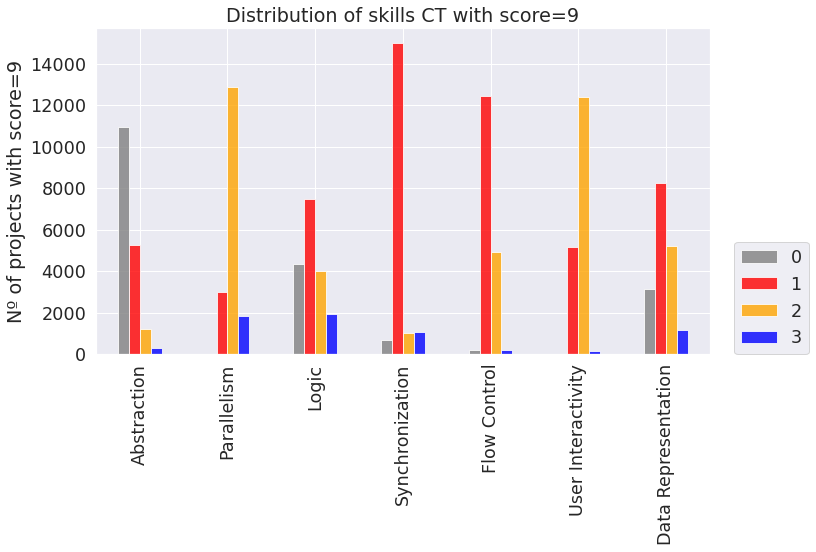
\includegraphics[width=\textwidth]{img/distribucion_9_Scratch}
        \caption{Diagrama de barras. Total=9}
        \label{fig:total9}
    \end{subfigure}       
    \begin{subfigure}[h]{.49\textwidth} 
        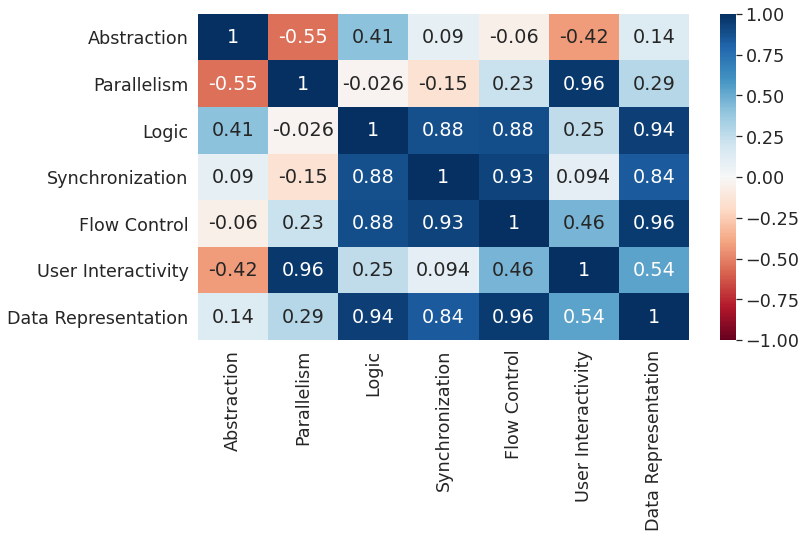
\includegraphics[width=\textwidth]{img/corr_9_Scratch}
        \caption{Matriz de correlación. Total=9}
        \label{fig:corr9}
    \end{subfigure}
     \caption{Distribución de puntuaciones asignadas y correlación entre dimensiones del PC cuando la puntuación total vale 9}
\end{figure}

Para la puntuación total de 10, en el diagrama de barras~\ref{fig:total10} aumenta la obtención de 2 puntos en lógica y de 3 puntos en representación de los datos, por el uso de listas. 

Existe una correlación perfecta directa entre lógica y paralelismo. Se consigue también una alta correlación positiva entre lógica e interactividad con el usuario y entre esta última y paralelismo. No hay dependencia lineal entre control de flujo y abstracción, ni entre sincronización y lógica, ni entre sincronización y paralelismo. Igual que en la puntuación anterior se obtiene una correlación moderada en sentido negativo entre abstracción y paralelismo. La capacidad de dividir el problema en partes sencillas de implementar y depurar, debería ayudar a descubrir cuáles de estas partes pueden ser ejecutadas de manera simultánea o concurrente, con una adecuada sincronización. Sin embargo el aumento de una habilidad hace que disminuya la otra. Además ambas son independientes de sincronización puesto que solo se usan bloques de espera. % %disminuye la ejecución de tareas de manera simultánea. según los datos analizados hasta ahora

\begin{figure}[H]
    \centering
    \begin{subfigure}[h]{.49\textwidth} 
        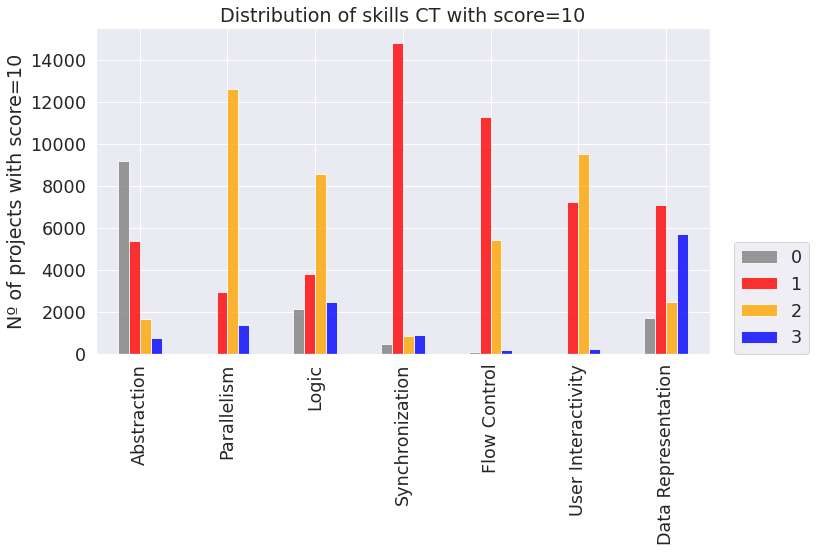
\includegraphics[width=\textwidth]{img/distribucion_10_Scratch}
        \caption{Diagrama de barras. Total=10}
        \label{fig:total10}
    \end{subfigure}       
    \begin{subfigure}[h]{.49\textwidth} 
        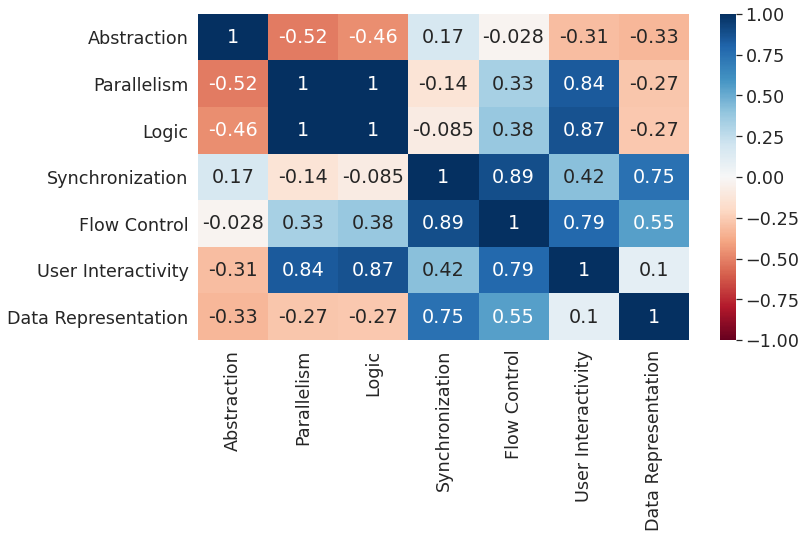
\includegraphics[width=\textwidth]{img/corr_10_Scratch}
        \caption{Matriz de correlación. Total=10}
        \label{fig:corr10}
    \end{subfigure}
     \caption{Distribución de puntuaciones asignadas y correlación entre dimensiones del PC cuando la puntuación total vale 10}
\end{figure}

\begin{figure}[H]
    \centering
    \begin{subfigure}[h]{.49\textwidth} 
        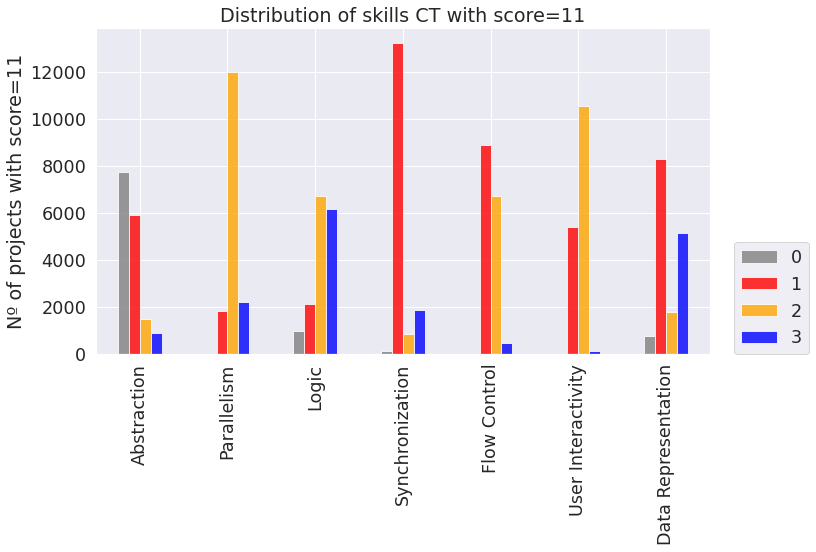
\includegraphics[width=\textwidth]{img/distribucion_11_Scratch}
        \caption{Diagrama de barras. Total=11}
        \label{fig:total11}
    \end{subfigure}       
    \begin{subfigure}[h]{.49\textwidth} 
        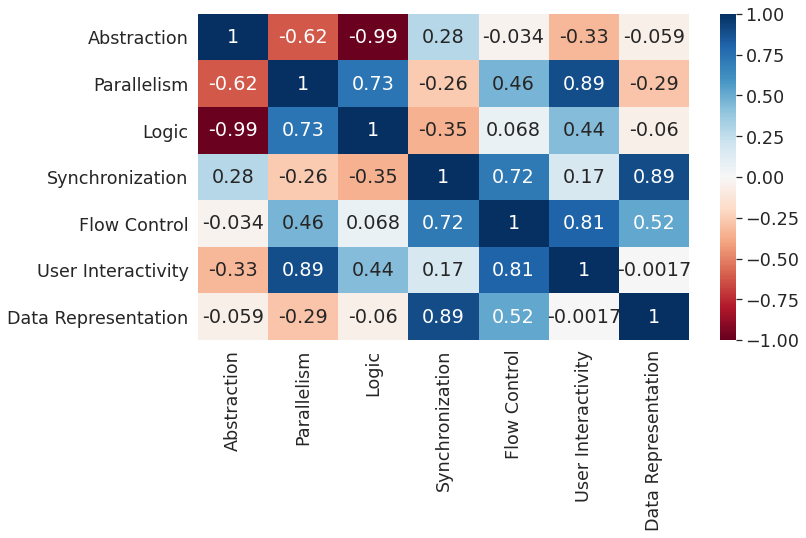
\includegraphics[width=\textwidth]{img/corr_11_Scratch}
        \caption{Matriz de correlación. Total=11}
        \label{fig:corr11}
    \end{subfigure}
     \caption{Distribución de puntuaciones asignadas y correlación entre dimensiones del PC cuando la puntuación total vale 11}
\end{figure}

Para la puntuación total de 11, en el diagrama de barras~\ref{fig:total11} destaca el aumento de proyectos que consiguen 3 puntos en pensamiento lógico.

En la matriz de correlación~\ref{fig:corr11} se observan valores elevados entre interactividad con el usuario y paralelismo, entre sincronización y representación de los datos y entre control de flujo con interactividad con el usuario. Son independientes linealmente: control de flujo y abstracción, representación de los datos y abstracción, lógica y representación de los datos, lógica y control de flujo, interactividad del usuario y representación de los datos. Vuelve a existir correlación en sentido negativo entre paralelismo y abstracción. También se da una correlación negativa prácticamente perfecta entre lógica y abstracción. Al aumentar el uso de estructuras selectivas que pueden incluir operadores lógicos, disminuye la capacidad para plantear soluciones a problemas descomponiéndolos en scripts o funciones encargadas de tareas concretas que pueden ser reutilizadas cuando se extrae lo relevante, se reconocen patrones y se generaliza. % Evolución de la programación estructura a la modular

Para la puntuación de 12, según la matriz~\ref{fig:corr12}, existe una correlación elevada directa entre lógica y paralelismo, y entre paralelismo e interactividad con el usuario. Por ello cuando el usuario pulsa una tecla o un objeto se desencadena la ejecución de varias tareas a la vez. Se da una correlación positiva menor entre sincronización y abstracción y entre interactividad con el usuario y lógica. No hay correlación entre sincronización e interactividad con el usuario. La correlación en sentido negativo entre paralelismo y abstracción se aproxima a -1, mientras que entre lógica y abstracción es fuerte pero no perfecta, comparada con la puntuación anterior. %% Paralelismo e interactividad con el usuario cont $\rho\simeq1 $


\begin{figure}[H]
    \centering
    \begin{subfigure}[h]{.49\textwidth} 
        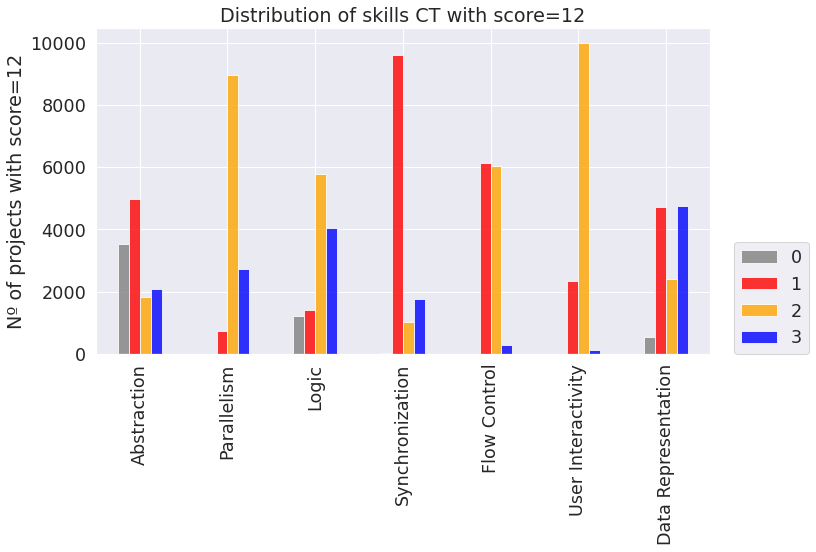
\includegraphics[width=\textwidth]{img/distribucion_12_Scratch}
        \caption{Diagrama de barras. Total=12}
        \label{fig:total12}
    \end{subfigure}       
    \begin{subfigure}[h]{.49\textwidth} 
        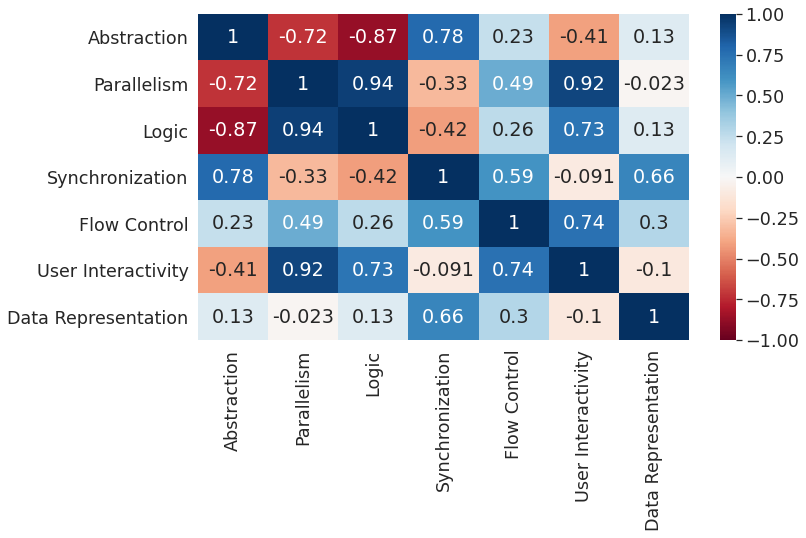
\includegraphics[width=\textwidth]{img/corr_12_Scratch}
        \caption{Matriz de correlación. Total=12}
        \label{fig:corr12}
    \end{subfigure}
     \caption{Distribución de puntuaciones asignadas y correlación entre dimensiones del PC cuando la puntuación total vale 12}
\end{figure}

Para la puntuación total de 13, el diagrama de barras~\ref{fig:total13} refleja un aumento en el uso de clones o instancias de los personajes creadas dinámicamente con el mismo comportamiento que el objeto inicial, como se infiere de la cantidad de proyectos con 3 puntos en abstracción.

En la matriz~\ref{fig:corr13} se obtiene una correlación positiva fuerte entre sincronización y abstracción, entre paralelismo e interactividad con el usuario, entre lógica y paralelismo %viene desde 10
y entre representación de los datos y abstracción. Al declarar atributos y listas y modificar su contenido se abstraen características de los personajes y se agrupan datos que pueden ser procesados por una misma secuencia de instrucciones o programa. No existe dependencia lineal entre interactividad del usuario con sincronización, entre control de flujo y representación de los datos, ni entre lógica y abstracción. Se recogen estos coeficientes en la figura~\ref{fig:corr13}. %La dependencia lineal inversa entre paralelismo y abstracción es más débil que en las matrices de correlación anteriores. 

\begin{figure}[H]
    \centering
    \begin{subfigure}[h]{.49\textwidth} 
        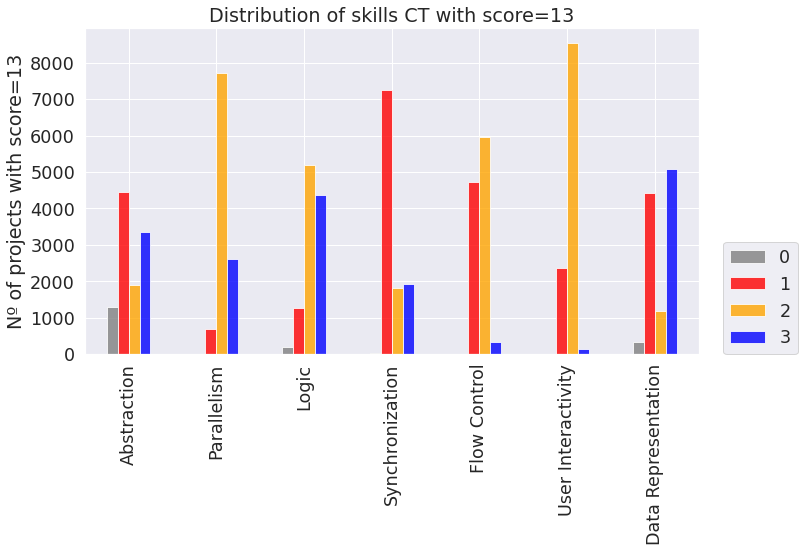
\includegraphics[width=\textwidth]{img/distribucion_13_Scratch}
        \caption{Diagrama de barras. Total=13}
        \label{fig:total13}
    \end{subfigure}       
    \begin{subfigure}[h]{.49\textwidth} 
        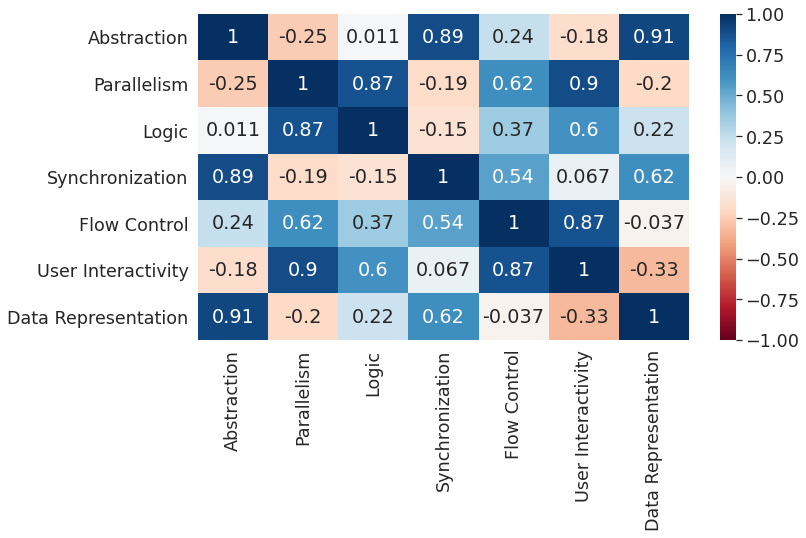
\includegraphics[width=\textwidth]{img/corr_13_Scratch}
        \caption{Matriz de correlación. Total=13}
        \label{fig:corr13}
    \end{subfigure}
     \caption{Distribución de puntuaciones asignadas y correlación entre dimensiones del PC cuando la puntuación total vale 13}
\end{figure}

Para la puntuación total de 14, en el diagrama de barras~\ref{fig:total14} la puntuación más frecuente en lógica es 3. En los proyectos que la consiguen 
se evalúan varias situaciones utilizando operadores lógicos, que permiten elegir entre distintas alternativas, obteniendo salidas diferentes.% se decide entre distintas alternativas en base a situaciones, premisas o condiciones.

En la matriz~\ref{fig:corr14} se observa una correlación positiva casi perfecta entre control de flujo e interactividad con el usuario. La dependencia lineal es elevada y positiva entre: paralelismo e interactividad con el usuario, representación de los datos con abstracción, control de flujo con paralelismo y lógica con paralelismo. Interactividad del usuario y sincronización son incorreladas, indicando que la gestión de las respuestas del usuario ante determinadas preguntas, de los movimientos con el ratón sobre objetos o de cómo responde el programa cuando se pulsa una tecla, no afecta a la capacidad del programador para planificar el orden en que se ejecutan las distintas tareas de modo que interactúen entre sí.%%

\begin{figure}[H]
    \centering
    \begin{subfigure}[h]{.49\textwidth} 
        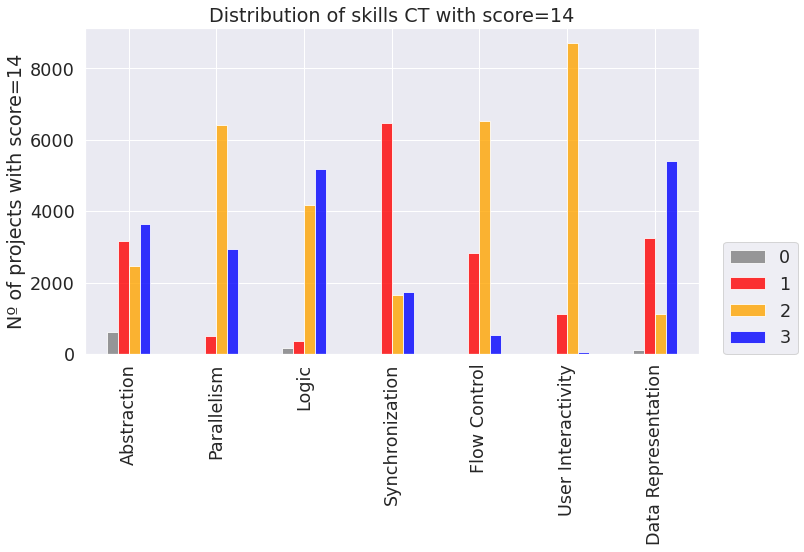
\includegraphics[width=\textwidth]{img/distribucion_14_Scratch}
        \caption{Diagrama de barras. Total=14}
        \label{fig:total14}
    \end{subfigure}       
    \begin{subfigure}[h]{.49\textwidth} 
        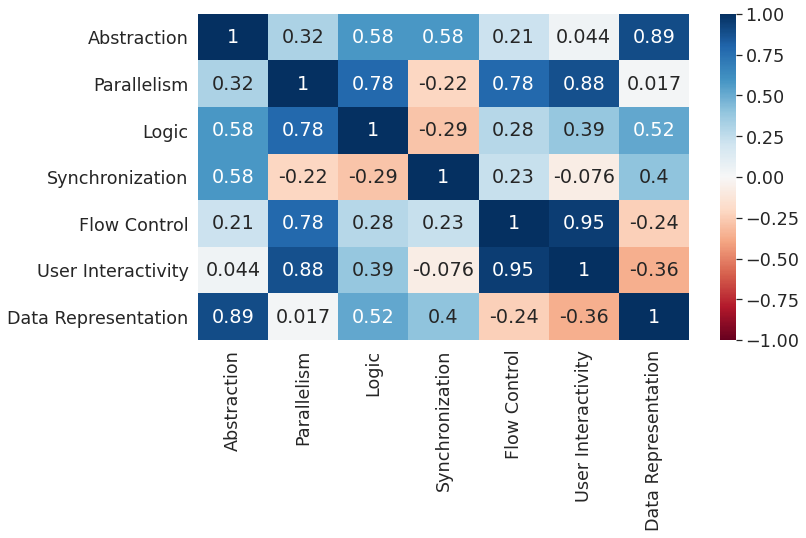
\includegraphics[width=\textwidth]{img/corr_14_Scratch}
        \caption{Matriz de correlación. Total=14}
        \label{fig:corr14}
    \end{subfigure}
     \caption{Distribución de puntuaciones asignadas y correlación entre dimensiones del PC cuando la puntuación total vale 14}
\end{figure}

\begin{figure}[H]
    \centering
    \begin{subfigure}[h]{.49\textwidth} 
        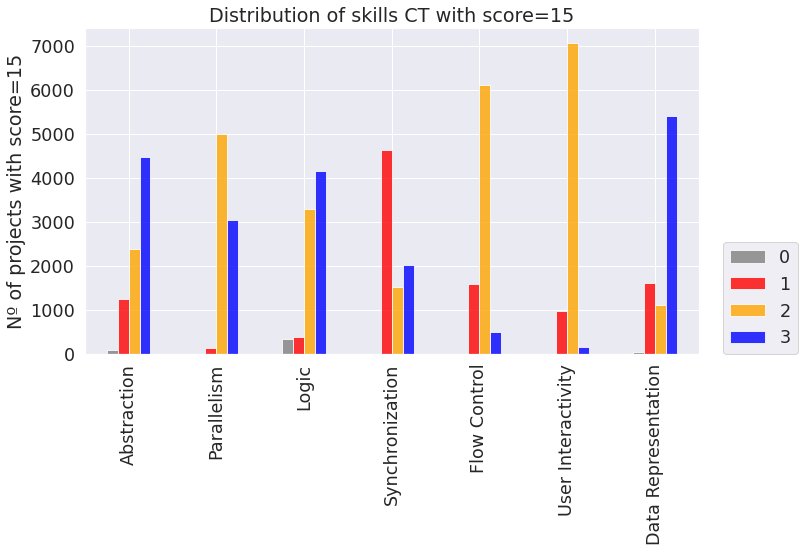
\includegraphics[width=\textwidth]{img/distribucion_15_Scratch}
        \caption{Diagrama de barras. Total=15}
        \label{fig:total15}
    \end{subfigure}       
    \begin{subfigure}[h]{.49\textwidth} 
        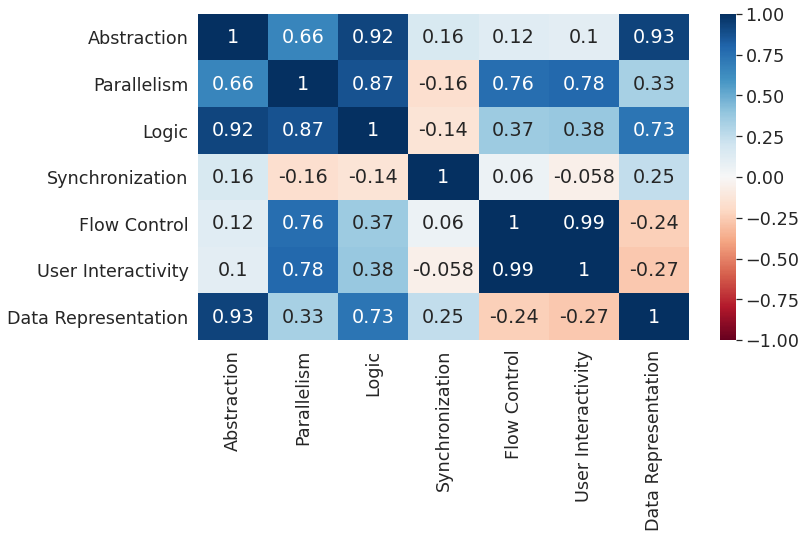
\includegraphics[width=\textwidth]{img/corr_15_Scratch}
        \caption{Matriz de correlación. Total=15}
        \label{fig:corr15}
    \end{subfigure}
     \caption{Distribución de puntuaciones asignadas y correlación entre dimensiones del PC cuando la puntuación total vale 15}
\end{figure}

Con respecto a la puntuación total de 15, en el diagrama de barras~\ref{fig:total15} se percibe un incremento en las frecuencias correspondientes a los 3 puntos tanto en abstracción, al emplear clones, como en representación de los datos, por utilizar listas.

La matriz de correlación~\ref{fig:corr15} muestra una dependencia lineal directa perfecta entre control de flujo con interactividad con el usuario, y una correlación positiva muy elevada entre lógica y abstracción, entre representación de los datos y abstracción, entre lógica y paralelismo, entre interactividad con el usuario y paralelismo y entre control de flujo y paralelismo. Como en otras puntuaciones anteriores, sincronización e interactividad con el usuario, abstracción e interactividad con el usuario y control de flujo y sincronización están incorreladas.%%

En la puntuación total de 16 se consigue que la máxima puntuación sea la más frecuente en abstracción, \emph{lógica} y representación de los datos. En paralelismo, control de flujo e interactividad con el usuario persisten los 2 puntos, como se constata en el diagrama~\ref{fig:total16}.

Según la figura~\ref{fig:corr16} se producen elevadas dependencias en sentido positivo, ordenadas de mayor a menor, entre interactividad del usuario y control de flujo, entre lógica y paralelismo, entre abstracción y representación de los datos, entre lógica y abstracción y entre paralelismo y abstracción. La dependencia lineal de este último par ha cambiado de sentido con respecto a las 12 primeras puntuaciones totales, de manera que al aumentar la capacidad para dar modularidad al código y utilizar clones, se incrementa la habilidad de discernir qué funciones y procedimientos pueden ejecutarse simultáneamente cuando se produzca un evento. No existe correlación entre control de flujo y sincronización, ni entre interactividad del usuario y sincronización, ni entre control de flujo y abstracción, ni entre interactividad del usuario y abstracción, ni entre paralelismo y sincronización, ni entre lógica y sincronización.

\begin{figure}[H]
    \centering
    \begin{subfigure}[h]{.49\textwidth} 
        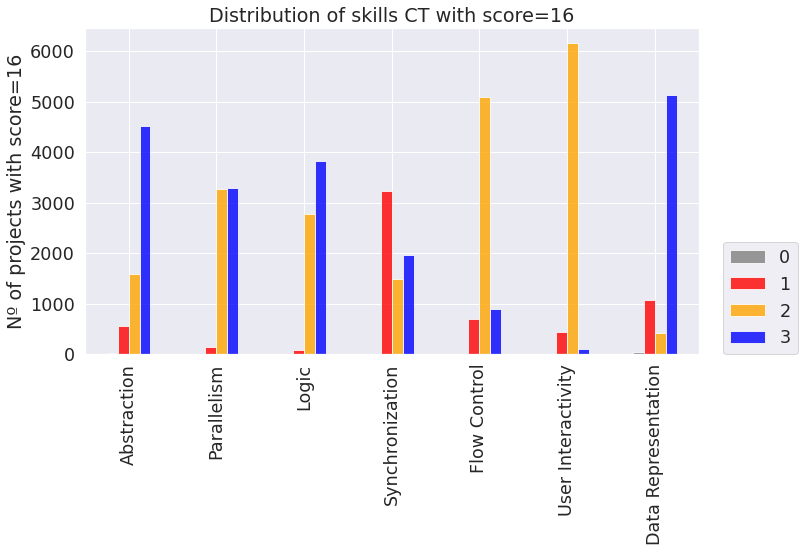
\includegraphics[width=\textwidth]{img/distribucion_16_Scratch}
        \caption{Diagrama de barras. Total=16}
        \label{fig:total16}
    \end{subfigure}       
    \begin{subfigure}[h]{.49\textwidth} 
        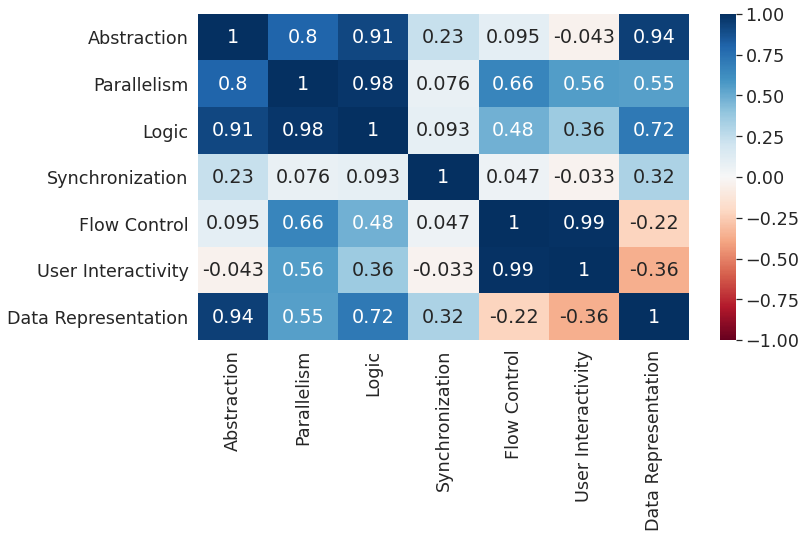
\includegraphics[width=\textwidth]{img/corr_16_Scratch}
        \caption{Matriz de correlación. Total=16}
        \label{fig:corr16}
    \end{subfigure}
     \caption{Distribución de puntuaciones asignadas y correlación entre dimensiones del PC cuando la puntuación total vale 16}
\end{figure}

Con respecto a la puntuación total de 17, mientras que abstracción, \emph{paralelismo}, lógica y representación de datos están prácticamente desarrolladas, control de flujo e interactividad del usuario se mantienen en los 2 puntos, como se aprecia en la figura~\ref{fig:total17}. La cantidad de proyectos de Scratch que consiguen 1 y 3 puntos en sincronización es similar.

Según se muestra en la matriz de correlación~\ref{fig:corr17}
se establecen interdependencias lineales perfectas directas entre las capacidades con 3 puntos, de manera que al descomponer en partes más sencillas el problema definiendo funciones propias o creando dinámicamente clones de los personajes, 
se ejecutan simultáneamente varios flujos de código o programas y en algunos de ellos se emplean condicionales con operadores lógicos para decidir el conjunto de instrucciones a ejecutar y cómo se modifican los datos contenidos en listas.
% se incrementa la capacidad de establecer cuáles de estas partes permiten su ejecución simultánea,
No existe dependencia lineal entre control de flujo y abstracción, entre control de flujo y sincronización, ni entre interactividad del usuario y la mayor parte de las dimensiones, salvo control de flujo, porque cuando se crean programas interactivos aumenta la capacidad de diseñar y aplicar algoritmos iterativos. %%% Versión mas teórica al estar en 3, revisar.

\begin{figure}[H]
    \centering
    \begin{subfigure}[h]{.49\textwidth} 
        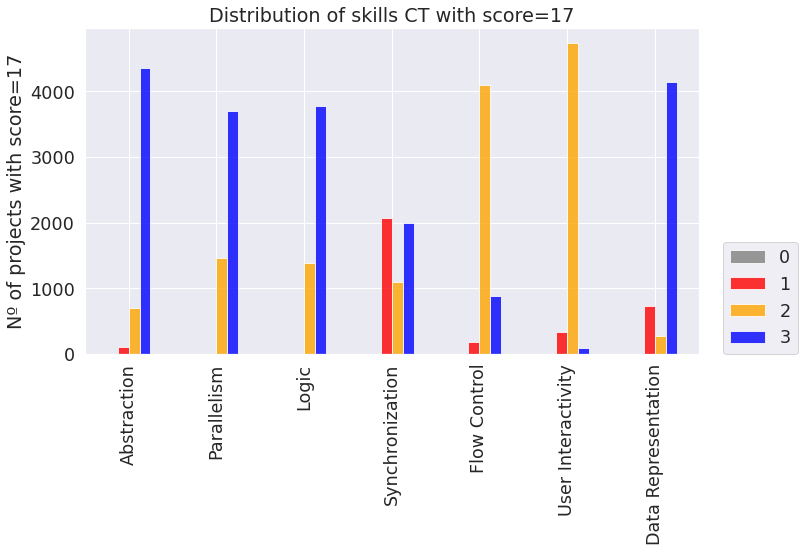
\includegraphics[width=\textwidth]{img/distribucion_17_Scratch}
        \caption{Diagrama de barras. Total=17}
        \label{fig:total17}
    \end{subfigure}       
    \begin{subfigure}[h]{.49\textwidth} 
        \includegraphics[width=\textwidth]{img/corr_17_Scratch}
        \caption{Matriz de correlación. Total=17}
        \label{fig:corr17}
    \end{subfigure}
     \caption{Distribución de puntuaciones asignadas y correlación entre dimensiones del PC cuando la puntuación total vale 17}
\end{figure}

El paso de los 17 a los 18 puntos totales está marcado por el desarrollo casi completo de la sincronización, como se deduce al comparar los diagramas de barras~\ref{fig:total17} y ~\ref{fig:total18}.

Se conservan las correlaciones casi perfectas explicadas en la puntuación anterior y se añaden las que surgen entre sincronización con las otras habilidades evaluadas con 3 puntos. Por ello cuando se establece previamente el orden en que los programas serán ejecutados, de forma que interactúen y se comuniquen entre sí con mensajes, eventos o esperando el resultado de algún script, resulta más fácil que las distintas partes en que se descompone el problema puedan ejecutarse en paralelo, empleen estructuras selectivas que indiquen por donde continúa el flujo del programa y se utilicen métodos propios de listas para modificar los datos que contiene, que a su vez pueden ser usados como condiciones o eventos. Existe una correlación positiva baja entre control de flujo y lógica. Entre cada par de variables no comentadas, se puede decir que no existe correlación. Todo esto queda reflejado en la matriz~\ref{fig:corr18}.

\begin{figure}[H]
    \centering
    \begin{subfigure}[h]{.49\textwidth} 
        \includegraphics[width=\textwidth]{img/distribucion_18_Scratch}
        \caption{Diagrama de barras. Total=18}
        \label{fig:total18}
    \end{subfigure}       
    \begin{subfigure}[h]{.49\textwidth} 
        \includegraphics[width=\textwidth]{img/corr_18_Scratch}
        \caption{Matriz de correlación. Total=18}
        \label{fig:corr18}
    \end{subfigure}
     \caption{Distribución de puntuaciones asignadas y correlación entre dimensiones del PC cuando la puntuación total vale 18}
\end{figure}

\begin{figure}[H]
    \centering
    \begin{subfigure}[h]{.49\textwidth} 
        \includegraphics[width=\textwidth]{img/distribucion_19_Scratch}
        \caption{Diagrama de barras. Total=19}
        \label{fig:total19}
    \end{subfigure}       
    \begin{subfigure}[h]{.49\textwidth} 
        \includegraphics[width=\textwidth]{img/corr_19_Scratch}
        \caption{Matriz de correlación. Total=19}
        \label{fig:corr19}
    \end{subfigure}
     \caption{Distribución de puntuaciones asignadas y correlación entre dimensiones del PC cuando la puntuación total vale 19}
\end{figure}

Cuando la complejidad de los proyectos alcanza los 19 puntos, control de flujo e interactividad con el usuario siguen en 2 puntos, y el resto de dimensiones se perfilan aún más en los 3 puntos, marcando un desarrollo completo (ver figura~\ref{fig:total19}).

Debido a esta distribución de puntuaciones, las matrices de correlación~\ref{fig:corr18} y~\ref{fig:corr19} muestran las mismas correlaciones perfectas positivas. Control de flujo es independiente linealmente de las otras dimensiones, salvo de interactividad con el usuario. Interactividad con el usuario presenta correlaciones inversas bajas y moderadas con el resto  de dimensiones.

Para la puntuación total de 20, control de flujo logra alcanzar la máxima puntuación al utilizarse bucles en donde se itera hasta que se cumple una condición.

La correlación es perfecta positiva entre todas las dimensiones del pensamiento computacional, salvo para interactividad con el usuario con el resto de dimensiones, como vemos en la matriz~\ref{fig:corr20}. Esto se debe a que, según vemos en el diagrama de barras~\ref{fig:total20}, las puntuaciones de la mayor parte de los proyectos para interactividad con el usuario son de 2 puntos. Por ello su correlación es perfecta negativa con cada una de las otras áreas del PC. 

\begin{figure}[H]
    \centering
    \begin{subfigure}[h]{.49\textwidth} 
        \includegraphics[width=\textwidth]{img/distribucion_20_Scratch}
        \caption{Diagrama de barras. Total=20}
        \label{fig:total20}
    \end{subfigure}       
    \begin{subfigure}[h]{.49\textwidth} 
        \includegraphics[width=\textwidth]{img/corr_20_Scratch}
        \caption{Matriz de correlación. Total=20}
        \label{fig:corr20}
    \end{subfigure}
     \caption{Distribución de puntuaciones asignadas y correlación entre dimensiones del PC cuando la puntuación total vale 20}
\end{figure}

Por lo tanto la última dimensión en desarrollarse por completo es interactividad con el usuario como se deduce al comparar las distribuciones~\ref{fig:total20} y ~\ref{fig:total21}. El cambio de los 2 a los 3 puntos se produce por implementar acciones en los personajes que respondan a las modificaciones en el audio y el vídeo que realiza el usuario para interactuar con el proyecto de Scratch, aunque en el conjunto de proyectos analizado no se aplica demasiado. Resulta llamativo que sea de las primeras habilidades en manifestarse y de las últimas en completarse, y que mantenga dependencias lineales con control de flujo desde los 10 puntos totales %
y con paralelismo hasta los 15 puntos totales. No obstante, con paralelismo comparte métricas similares, puesto que se ejecutan varios programas simultáneamente al pulsar sobre objetos, teclas o la bandera verde, que son acciones valoradas con 1 y 2 puntos en interactividad con el usuario. %%Revisar
% Las correlaciones según aumenta la puntuación total no tienen coincidencias con la correlación general de las 7 dimensiones. 
% Sincronización y paralelismo deberían mostrar dependencias.

\subsection{Aprendizaje no supervisado: clustering K-Means con los proyectos de Scratch}
\label{subsec:kmeans_Scratch}

%Para profundizar en cómo se relacionan entre sí los proyectos en función de las siete dimensiones, se buscan patrones entre los mismos que nos ayuden a descubrir similitudes entre los proyectos basados en relaciones entre las habilidades, que no han podido establecerse a partir del estudio de las correlaciones. Aplicación de un modelo de ML aunque forma parte de un EDA al tratar de descubrir más info de los proyectos\ldots
Se utiliza este algoritmo de aprendizaje no supervisado, para dividir los 269842 proyectos de Scratch en subconjuntos no solapados o particiones. Se obtienen grupos de manera que los proyectos dentro de un clúster son muy similares, y totalmente distintos a los proyectos que pertenecen a otros grupos. La semejanza o diferencia se mide en función de la distancia euclídea a un centroide del clúster, que a partir de cierto nº de iteraciones, se colocará en el centro del clúster. K-Means trata de minimizar las distancias intra-partición y maximiza las distancias inter-partición.

% Matriz de dimensión (269842, 7)
La entrada al algoritmo es un array de vectores con tantas filas como observaciones o proyectos de Scratch y cuyas componentes son las características o dimensiones del pensamiento computacional. Como cada proyecto queda representado por un punto en un espacio de 7 dimensiones cuyas coordenadas son los valores de las puntuaciones asignadas a cada habilidad, al aplicar el algoritmo K-Means, y minimizarse las distancias al punto medio o centroide de cada clúster, la cohesión del grupo determina relaciones y patrones entre las habilidades difícilmente identificables de otro modo, como en el análisis previo de las correlaciones. 

Para aplicar K-Means es necesario conocer a priori el valor de k, el nº de grupos o centroides. Una de las técnicas más extendidas para estimarlo es la curva de Elbow. Se itera sobre un conjunto de posibles valores de k buscando un cambio abrupto en la inercia, de forma que un aumento en el valor de k no suponga una disminución significativa en dicha inercia. La inercia se define como la suma de las distancias euclídeas de cada punto con respecto al centroide o centro del clúster al que pertenece, como se indica en la ecuación~\eqref{eq:inercia}. %Se establece un compromiso entre un mínimo valor de inercia y una cantidad de grupos no muy elevado.

\begin{equation}
	Inercia=WCSS=\sum \limits _{i=0}^{N} \|{x_i-c_i\|^2}
	\label{eq:inercia}
\end{equation}

\begin{figure}
	\centering
	\includegraphics[width=.6\textwidth]{img/elbow_Scratch}
	\caption{Curva de Elbow}
	\label{fig:elbow_Scratch}
\end{figure}

% En metodología o en otra parte más teórica. 
La curva de Elbow de la figura~\ref{fig:elbow_Scratch} comienza a suavizarse a partir de k=3. Se entrena el algoritmo con este valor de k. El algoritmo coloca 3 centroides de manera aleatoria y tras varias iteraciones en que se asigna cada proyecto al centroide más cercano y se recalcula la posición de este centro en función de la media de los proyectos pertenecientes al grupo, llega un momento en que el algoritmo converge. Los centroides no cambian de posición porque no se modifican los proyectos pertenecientes a cada grupo o porque se ha alcanzado el nº máximo de iteraciones. Los proyectos son etiquetados según el clúster en el que están incluidos. Cada clúster queda descrito por el proyecto más cercano a su centroide o proyecto representativo. %siendo más fácil establecer patrones.

En el artículo~\cite{moreno17:_paths} se establece un itinerario de aprendizaje en tres pasos, de complejidad incremental, basado en los proyectos representativos o prototipos de los 3 clústeres obtenidos de una muestra de 250 proyectos tomadas del repositorio de Scratch. Se propuso comparar esos prototipos con los proyectos representativos de los 3 clústeres conseguidos en nuestro dataset.  

\begin{table}[H]
	\begin{subtable}[h]{0.49\textwidth}
		\centering
		\begin{tabular}{lrrr}
            {} & \multicolumn{3}{c}{\cellcolor[HTML]{FFCCC9}\textbf{Clúster}} \\ 
            \hline
            {} & \textbf{1} & \textbf{2} & \textbf{3} \\ 
            \hline
            \textbf{Pensamiento lógico} & 0 & 2 & 2 \\
            \textbf{Abstracción} & 0 & 0 & 3 \\
            \textbf{Interactividad con el usuario} & 1 & 2 & 2 \\
            \textbf{Representación de los datos} & 0 & 2 & 2 \\
            \textbf{Paralelismo} & 1 & 2 & 3 \\
            \textbf{Sincronización} & 1 & 1 & 2 \\
            \textbf{Control de flujo} & 1 & 1 & 2 \\ 
            \hline
            \textbf{Total} & 4 & 10 & 16 \\ 
            \hline
            \end{tabular}
            \caption{Dataset de 269842 proyectos}
		\label{table:prototype_269842}
	\end{subtable}
	~
	\begin{subtable}[h]{0.49\textwidth}
		\centering
		\begin{tabular}{lrrr}
			{\color[HTML]{000000} {}} & \multicolumn{3}{c}{\cellcolor[HTML]{CBCEFB}\textbf{Clúster}} \\ 
			\hline
			{} & \textbf{1} & \textbf{2} & \textbf{3} \\ \hline
			\textbf{Pensamiento lógico} & 0 & 0 & 3 \\
			\textbf{Abstracción} & 1 & 1 & 3 \\
			\textbf{Interactividad con el usuario} & 1 & 1 & 2 \\
			\textbf{Representación de los datos} & 1 & 1 & 2 \\
			\textbf{Paralelismo} & 1 & 3 & 3 \\
			\textbf{Sincronización} & 1 & 2 & 3 \\
			\textbf{Control de flujo} & 2 & 2 & 2 \\ 
			\hline
            \textbf{Total} & 7 & 10 & 18 \\ 
            \hline
		\end{tabular}
		\caption{Muestra de 250 proyectos}
		\label{table:prototype_250}
	\end{subtable}
	\caption{Similitud entre proyectos representativos de los 3 clústeres tras aplicar K-Means}
\end{table}

%Si haces tres clústeres (con K-Means, por ejemplo), ¿los proyectos representativos de cada clúster son similares a los que obtuvimos en el paper (ver Tabla 4 del paper)?
Para el clúster 1 de la tabla~\ref{table:prototype_269842} tenemos una puntuación total de 4 en el nivel básico, con un punto en las siguientes habilidades: interactividad con el usuario, paralelismo, sincronización y control de flujo. Se corresponde con un proyecto con 2 scripts que comienzan a e ejecutarse al pulsar la bandera verde, incluyen un bloque de espera y su flujo de ejecución es secuencial. En la tabla~\ref{table:prototype_250} se alcanzan 7 puntos totales para el clúster 1. Difiere en que se consigue 1 punto en abstracción y en representación de los datos, y 2 puntos en control de flujo por emplear bucles infinitos. Que se consiga menos puntuación tiene sentido, ya que en el estudio~\cite{moreno17:_paths} se estableció como requisito una complejidad mínima de 3 puntos totales para los proyectos de la muestra. No se tienen en cuenta los proyectos no completados que aquí sí se consideran.

Para el clúster 2, en el patrón establecido por el prototipo de nivel intermedio de nuestro dataset~\ref{table:prototype_269842}, se refuerzan tanto interactividad con el usuario como paralelismo, pues hay varios programas que se ejecutan simultáneamente al pulsar sobre un objeto o sobre una tecla (2 puntos). Se emplean variables para almacenar los datos de entrada que son procesados por los programas y se decide entre distintas salidas según se cumpla o no una condición, desarrollándose tanto la representación de los datos como el pensamiento lógico, que serían los núcleos de esta fase de aprendizaje.
En la tabla~\ref{table:prototype_250}, el proyecto que describe el clúster 2 logra la misma puntuación total (10 puntos), pero se progresa en habilidades distintas, concretamente en paralelismo y sincronización por el intercambio de mensajes entre varios personajes, con 3 y 2 puntos respectivamente. El resto de destrezas conservan las mismas puntuaciones que en el clúster 1.

El proyecto representativo del clúster 3 marca un nivel avanzado de 16 puntos, como se refleja en la tabla~\ref{table:prototype_269842}. Se consigue un notable progreso al hacer que varios personajes puedan intercambiar mensajes para ejecutar sentencias de manera concurrente. Se emplean clones que muestran una capacidad avanzada en abstracción y bucles por los que se obtiene 2 puntos en control de flujo. En la tabla~\ref{table:prototype_250}, el prototipo de la última fase en el itinerario establecido muestra una complejidad de 18 puntos en vez de 16. El aumento de 2 puntos se debe a que se cuenta con mecanismos avanzados de sincronización y con operadores lógicos para evaluar condiciones, propios de un alto desarrollo del pensamiento lógico. Es el clúster que más se parece al obtenido en nuestro análisis. La variación incremental se debe a que aquí se tienen en cuenta todos los proyectos, incluidos áquellos que están en progreso, para que el programador los mejore y en el artículo se seleccionó una muestra de proyectos con cierto nivel de elaboración.


\subsection{Análisis de clustering entre niveles o puntuaciones totales. Ruta de aprendizaje demostrada en los proyectos de Scratch}
\label{subsec:ruta_Scratch}

En base al itinerario de aprendizaje en 3 etapas basado en prototipos propuesto en el apartado~\ref{subsec:kmeans_Scratch}, se  busca conocer en detalle el proceso de aprendizaje demostrado por los proyectos de Scratch analizados que conforman nuestro dataset. 
En el estudio de las distribuciones por puntuaciones asignadas a las habilidades del PC del apartado~\ref{subsec:corr_21_Scratch}, se vislumbraba, en algunos casos, una única dimensión cuyo desarrollo provocaba el salto al siguiente nivel de complejidad o puntuación total. Sin embargo en la mayoría de ellos no era tan evidente. Tampoco quedaba claro qué combinación de dimensiones conformaba la puntuación total. 
Aunque sí se podía percibir qué capacidades comienzan a adquirirse antes, cuáles después y estimar cuál es su evolución conjunta e individualizada según se incrementa la dificultad.

Para responder de una manera más precisa a estas cuestiones, se agrupan de nuevo los proyectos según su puntuación total, aplicando el algoritmo clustering K-Means a cada uno de los 22 grupos. Se haya el proyecto más representativo de cada grupo. 
Con ello se consigue determinar el camino de aprendizaje seguido y la habilidad cuya mejora provoca el cambio de una puntuación total a la siguiente, que se refleja en la figura~\ref{fig:path_Scratch}.


\begin{figure}[H]
	\centering
	\includegraphics[width=1\textwidth]{img/path_CT_Scratch1.png}
  	\caption{Ruta de aprendizaje de las dimensiones del PC en Scratch}\label{fig:path_Scratch}
\end{figure}

\begin{itemize}
 \item El cambio de nivel entre 0 y 1: La primera competencia desarrollada es interactividad con el usuario, ya que el programa cuenta con el bloque que inicia su ejecución al pulsar la bandera verde.
 \item El cambio de nivel entre 1 y 2: Como se veía en la distribución~\ref{fig:total2}, los proyectos con 2 puntos cuentan con 2 o más scripts que se ejecutan a la vez al activar la bandera verde.
 \item El cambio de nivel entre 2 y 3: Paralelismo incrementa su valor de 1 a 2 puntos, al incluir las opciones de pulsar una tecla o sobre un objeto como bloques que desencadenan la ejecución simultánea de varios programas o tareas cuando dicho evento se produce.
 \item El cambio de nivel entre 3 y 4: Se implementa cada programa como una sucesión finita y ordenada de pasos concretos y bien definidos, por lo que se empieza a comprender el concepto de algoritmo, y qué fallos acarrea una incorrecta secuenciación. Por ello se asigna un punto a control de flujo. Se define con mayor exactitud lo intuido al comparar las distribuciones~\ref{fig:total3} y~\ref{fig:total4}. 
 \item El cambio de nivel entre 4 y 5: Sincronización empieza a puntuar al usar bloques de espera que establecen el orden temporal en que se ejecutan las tareas de distintos hilos. %flujos de código.
 \item El cambio de nivel entre 5 y 6: Se modifican los atributos asignados a cada personaje u objeto del proyecto, por lo que se logra un punto en representación de los datos.
 \item El cambio de nivel entre 6 y 7: Se comienza a desarrollar el pensamiento lógico, de modo que se implementa una acción determinada sujeta a que se cumpla cierta condición o premisa.
 \item El cambio de nivel o puntuación total entre 7 y 8: Interactividad del usuario pasa a valer 2 puntos, como se indicaba en la distribución~\ref{fig:total8}. Los personajes u objetos son controlados por el teclado o por el ratón. Se gestiona como responde el programa cuando ocurren estos eventos provocados por el usuario.
 \item El cambio de nivel entre 8 y 9: Abstracción es la destreza más compleja y por ello la última en obtener un punto. Se extrae lo relevante de un problema y se descompone en tareas concretas, ejecutadas por varios personajes, más fáciles de implementar, depurar y mantener.
 \item El cambio de nivel entre 9 y 10: En este paso son varias las capacidades que experimentan cambios. Abstracción vuelve a los 0 puntos, mientras que representación de los datos consigue los 2 puntos al utilizar variables como contenedores de un dato que se modifica o que es evaluado para la ejecución de una secuencia de instrucciones. Se emplean por tanto, estructuras selectivas if-else que evalúan una condición determinando por dónde continúa el flujo del programa, y que acción debe llevarse a cabo. Por ello, en lógica se obtienen 2 puntos.
 \item El cambio de nivel entre 10 y 11: Abstracción recupera el punto al implementarse la solución del problema en varios programas más simples y para varios personajes.
 \item El cambio de nivel entre 11 y 12: Se utilizan bucles que repiten la ejecución de sentencias un nº determinado o indefinido de veces, reforzando la capacidad de control de flujo que consigue un nivel intermedio de desarrollo valorado con 2 puntos.
 \item El cambio de nivel entre 12 y 13: En abstracción se consiguen 2 puntos. El programador de Scratch define procedimientos o funciones propias que pueden ser reutilizadas en el objeto donde se crearon, llamándolas con los parámetros de entrada que se requieran. %se profundiza en el diseño algorítmico  Programación modular. Divide y vencerás. programación top-down. Al descomponer la solución del problema en programas ...  
 \item El cambio de nivel o puntuación total entre 13 y 14: Sincronización toma un valor de 2 puntos. Se emplean el intercambio de mensajes y mecanismos de parada para establecer el orden en que se ejecutan las acciones, de manera que los personajes y programas del proyecto interactúen entre sí.
 \item El cambio de nivel entre 14 y 15: Se declaran listas o estructuras de datos ordenadas, mutables y dinámicas, que almacenan un conjunto de strings o números, requeridos por el programa y cuyos valores son modificados por instrucciones propias de listas durante la ejecución del mismo. Por ello, representación de los datos es la primera capacidad completamente desarrollada y marca el paso al nivel avanzado.
 \item El cambio de nivel entre 15 y 16: Abstracción incrementa su valor a 3 puntos por el uso de clones, que son instancias de un objeto con los mismos atributos y métodos, creados dinámicamente cuando se necesitan varias copias del personaje original con el mismo comportamiento. Facilita el mantenimiento y la modificación del código. % diferente estado pues se puede modificar posición... 
 \item El cambio de nivel entre 16 y 17: Se utilizan operadores lógicos para evaluar condiciones y decidir si se ejecuta el código implementado asociado. Al combinar el diseño de algoritmos selectivos con la lógica booleana se consigue la máxima puntuación en pensamiento lógico. Paralelismo consigue también 3 puntos, pues se ejecutan simultáneamente varios scripts cuando reciben un mensaje, cambia el escenario o cuando se producen otros eventos multimedia. En representación de los datos se baja a los 2 puntos, pues se emplean variables para almacenar los datos con los que trabaja el programa y no listas.
 \item El cambio de nivel entre 17 y 18: De nuevo se declaran y modifican listas en los programas del proyecto de Scratch. 
 Por lo tanto, representación de los datos vuelve a valer 3 puntos.
 \item El cambio de nivel entre 18 y 19: Se establecen mecanismos de sincronización condicionales o basados en eventos, como el cambio de escenario. La ejecución de un programa continúa cuando se obtiene cierto resultado en otro proceso que envía los datos y espera que sean procesados para continuar con su flujo. Por ello, sincronización vale 3 puntos. %% Esperar hasta, cuando el fondo cambie a, enviar y esperar 

 \item El cambio de nivel entre 19 y 20: Control de flujo alcanza los 3 puntos, puesto que se refuerza la comprensión de los algoritmos iterativos al utilizar bucles sujetos a condiciones. Concuerda con lo obtenido en la distribución ~\ref{fig:total20}. % repetir hasta
 \item El cambio de nivel o puntuación total entre 20 y 21: Se implementan acciones a realizar por los objetos empleando bloques sensores que detectan cambios en la intensidad del sonido o movimiento cuando el usuario emplea el micrófono o la webcam para actuar sobre el proyecto. Interactividad del usuario es la última habilidad que se completa, como ya se indicó en el apartado~\ref{subsec:corr_21_Scratch}. 
\end{itemize}

\section{Análisis de datos de proyectos de Snap!} 
\label{sec:result_snap}
% Por lo demás, intenta siempre contar una historia: además de mostrar los resultados, que eso se os da bien, piensa en la motivación (por qué), en el método (cómo) y en las consecuencias (¿para qué?). 

A continuación se observa la distribución de proyectos de Snap!

\begin{figure}[H]
	\centering
  	\includegraphics[bb=0 0 800 600, width=11cm, keepaspectratio]{img/frequency_total_score.png}
  	\caption{Distribución de proyectos de Snap! por puntuación total.}\label{fig:total}
\end{figure}

% Se analiza si dichas valoraciones poseen una complejidad creciente con métricas discriminantes, que provoquen distribuciones decrecientes.
% Se desglosa en función de cada una de las siete dimensiones del PC  y se halla la distribución de proyectos para cada puntuación entera entre 0 y 3. 
% Se comprueba si las valoraciones establecidas representan una complejidad creciente que se traduzca en una distribución decreciente, de manera que la cantidad de proyectos que consiguen las puntuaciones más altas en cada dimensión desarrollada sea cada vez menor.


%ADATOS: Análisis multivariante:
%- resumir los datos con la mínima pérdida de información 
%-encontrar grupos en los datos si existen
%-clasificar nuevas observaciones en los grupos definidos.
%y relacionar dos conjuntos de variables, Entendimiento Grado de relación de 2 o más variables Gráfico de dispersión. Cuantificar o medir el grado de relación lineal entre dos variables, interdependencia, -1 1, invariante por transfomaciones lineales
% Eventos: Acciones programadas para ese evento concreto. Un evento dispara la ejecución de las sentencias que penden de él


Como se aprecia en la figura~\ref{fig:total} existe una mayor concentración de los proyectos entre las puntuaciones totales de 4 y 10 puntos. La moda se localiza en los 5 puntos. La distribución de frecuencias absolutas es representada a partir del diagrama de barras.

\begin{itemize}
    \item[•] ffff
\end{itemize}

\begin{figure}[H]
	\centering
	\includegraphics[width=1.0\textwidth]{img/path_CT_Snap.png}
  	\caption{Ruta de aprendizaje de las dimensiones del PC en Snap!}\label{fig:path_Snap}
\end{figure}

    

%%%%%%%%%%%%%%%%%%%%%%%%%%%%%%%%%%%%%%%%%%%%%%%%%%%%%%%%%%%%%%%%%%%%%%%%%%%%%%%%
%%%%%%%%%%%%%%%%%%%%%%%%%%%%%%%%%%%%%%%%%%%%%%%%%%%%%%%%%%%%%%%%%%%%%%%%%%%%%%%%
% CONCLUSIONES %
%%%%%%%%%%%%%%%%%%%%%%%%%%%%%%%%%%%%%%%%%%%%%%%%%%%%%%%%%%%%%%%%%%%%%%%%%%%%%%%%

\cleardoublepage
\chapter{Conclusiones}
\label{chap:conclusiones}


\section{Consecución de objetivos}
\label{sec:consecucion-objetivos}

Esta sección es la sección espejo de las dos primeras del capítulo de objetivos, donde se planteaba el objetivo general y se elaboraban los específicos.

Es aquí donde hay que debatir qué se ha conseguido y qué no. 
Cuando algo no se ha conseguido, se ha de justificar, en términos de qué problemas se han encontrado y qué medidas se han tomado para mitigar esos problemas.

Y si has llegado hasta aquí, siempre es bueno pasarle el corrector ortográfico, que las erratas quedan fatal en la memoria final.
Para eso, en Linux tenemos aspell, que se ejecuta de la siguiente manera desde la línea de \emph{shell}:

\begin{verbatim}
  aspell --lang=es_ES -c memoria.tex
\end{verbatim}

\section{Aplicación de lo aprendido}
\label{sec:aplicacion}

Aquí viene lo que has aprendido durante el Grado/Máster y que has aplicado en el TFG /TFM. 
Una buena idea es poner las asignaturas más relacionadas y comentar en un párrafo los conocimientos y habilidades puestos en práctica.

\begin{enumerate}
  \item a
  \item b
\end{enumerate}


\section{Lecciones aprendidas}
\label{sec:lecciones_aprendidas}

Aquí viene lo que has aprendido en el Trabajo Fin de Grado/Máster.

\begin{enumerate}
  \item Aquí viene uno.
  \item Aquí viene otro.
\end{enumerate}


\section{Trabajos futuros}
\label{sec:trabajos_futuros}

Ningún proyecto ni software se termina, así que aquí vienen ideas y funcionalidades que estaría bien tener implementadas en el futuro.

Es un apartado que sirve para dar ideas de cara a futuros TFGs/TFMs.


%%%%%%%%%%%%%%%%%%%%%%%%%%%%%%%%%%%%%%%%%%%%%%%%%%%%%%%%%%%%%%%%%%%%%%%%%%%%%%%%
%%%%%%%%%%%%%%%%%%%%%%%%%%%%%%%%%%%%%%%%%%%%%%%%%%%%%%%%%%%%%%%%%%%%%%%%%%%%%%%%
% APÉNDICE(S) %
%%%%%%%%%%%%%%%%%%%%%%%%%%%%%%%%%%%%%%%%%%%%%%%%%%%%%%%%%%%%%%%%%%%%%%%%%%%%%%%%

\cleardoublepage
\appendix
\chapter{Manual de usuario}
\label{app:manual}

Esto es un apéndice.
Si has creado una aplicación, siempre viene bien tener un manual de usuario.
Pues ponlo aquí.

%%%%%%%%%%%%%%%%%%%%%%%%%%%%%%%%%%%%%%%%%%%%%%%%%%%%%%%%%%%%%%%%%%%%%%%%%%%%%%%%
%%%%%%%%%%%%%%%%%%%%%%%%%%%%%%%%%%%%%%%%%%%%%%%%%%%%%%%%%%%%%%%%%%%%%%%%%%%%%%%%
% BIBLIOGRAFIA %
%%%%%%%%%%%%%%%%%%%%%%%%%%%%%%%%%%%%%%%%%%%%%%%%%%%%%%%%%%%%%%%%%%%%%%%%%%%%%%%%

\cleardoublepage

% Las siguientes dos instrucciones es todo lo que necesitas
% para incluir las citas en la memoria
\bibliographystyle{abbrv}
\bibliography{memoria}  % memoria.bib es el nombre del fichero que contiene
% las referencias bibliográficas. Abre ese fichero y mira el formato que tiene,
% que se conoce como BibTeX. Hay muchos sitios que exportan referencias en
% formato BibTeX. Prueba a buscar en http://scholar.google.com por referencias
% y verás que lo puedes hacer de manera sencilla.
% Más información: 
% http://texblog.org/2014/04/22/using-google-scholar-to-download-bibtex-citations/

\end{document}
